%Replace Strings:
%PROJECT.TITLE
%TODO.CHANGE
%PROJECT.ABSTRACT.KEYWORDS

\documentclass[12pt, a4paper, oneside]{article}

\usepackage[utf8]{inputenc}
\usepackage[bindingoffset=1.57cm, left=2.54cm, right=2.54cm, top=2.54cm, bottom=2.54cm]{geometry}
\usepackage{mathptmx}
\usepackage{fancyhdr}
\usepackage{appendix}
\usepackage{lipsum}
\usepackage{secdot}
\usepackage{lastpage}
\usepackage{tocloft}
\usepackage{cite}
\usepackage{tabularx}
\usepackage{booktabs}
\usepackage{pdflscape}
\usepackage{longtable}
\usepackage{enumitem}


\usepackage{geometry}
        \geometry{left=1in, right=1in, top=1in, bottom=1in}
\usepackage{graphicx}
	\graphicspath{ {images/} }
	
\usepackage{subcaption}
\usepackage{titlesec}
\usepackage{multirow}
\usepackage[hidelinks]{hyperref}

\usepackage{listings}
\usepackage{tocloft}
\usepackage[table,xcdraw]{xcolor}
\usepackage{floatrow}
\floatsetup[table]{capposition=bottom}

\usepackage{ltxtable}

\linespread{1.2}
\pagestyle{fancy}
\fancyhf{} % sets both header and footer to nothing
\renewcommand{\headrulewidth}{0pt}
\rhead{ \textit{FoodFind - A Restaurant Discovery Platform}}
\cfoot{\thepage}

\setlength{\parindent}{0pt}
\setlength{\parskip}{12pt}

\begin{document}


\pagenumbering{roman}


\addcontentsline{toc}{section}{Acknowledgement}
\large
\begin{center}
	\textbf{ACKNOWLEDGEMENT}
\end{center}
\normalsize
We would like to express our heartfelt gratitude to everyone who contributed to the successful completion of the FoodFind project, our innovative web application designed to enhance the dining experience.

First and foremost, we extend our sincere appreciation to our project supervisor, Mr. Bhusan Thapa, for his invaluable guidance and support throughout the project. Their expertise and constructive feedback played a pivotal role in shaping the direction and functionality of FoodFind.

Our gratitude also extends to Nepal College of Information Technology for providing us with the platform and resources to undertake this project. The opportunity to work on a real-world application enriched our learning experience and paved the way for our future endeavors.

We would also like to thank our teammates for their dedication, hard work, and collaboration. Each member's unique skills and efforts were crucial in bringing FoodFind to life.

In conclusion, the success of the FoodFind project would not have been possible without the support and contributions of our supervisor, teammates, and institution. We are immensely grateful for this opportunity and look forward to exploring new horizons in the world of technology and innovation.

\begin{flushleft}
Sincerely, \\
Bhok Lagyo Team
\end{flushleft}
\pagebreak


\addcontentsline{toc}{section}{Abstract}
\large
\begin{center}
	\textbf{ABSTRACT}
\end{center}
\normalsize
It is difficult to find delicious food at good restaurants in today's crowded city. Especially for those who are unfamiliar with places they have never been. FoodFind attempts to help those users in finding an appropriate place to eat near them. FoodFind is a webapp that helps users find restaurants and small businesses that match their tastes. FoodFind allows users to simply search for restaurants by name and location, as well as filter them depending on the food they provide. FoodFind allows users to see menus of different restaurants, see prices and see the variety of food items available. User's can also provide the reviews for the restaurants they visit. Which will help other users to know about the place. Additionally, users can also share the location of the restaurants they visited with others. FoodFind aims to help restaurants by showcasing them to other users that their food is best. FoodFind also includes filters to narrow down the user's choice based on food type, location and user reviews. This allows user to find exactly the place where they can enjoy their food. FoodFind is about connecting people with the quality food. A community where user's can share their love for the food and discover new places to try out as well tell others if the place is worth it or not. With FoodFind, every meal is an opportunity to explore and enjoy the city's rich flavours. 

\textbf{Keywords}: \textit{Web Application (Webapp), Hybrid Recommendation\\ 
RESTFUL APIs, MVC, RestaurantDiscovery}\\
\pagebreak
\break

\large
\addcontentsline{toc}{section}{Table of Contents}
\begin{center}
	\textbf{TABLE OF CONTENTS}
\end{center}
\normalsize
\setlength{\cftbeforetoctitleskip}{0pt}
\renewcommand{\contentsname}{}
\tableofcontents
\break


\large
\addcontentsline{toc}{section}{List of Figures}
\begin{center}
	\textbf{LIST OF FIGURES}
\end{center}
\renewcommand{\cftfigpresnum}{Figure }
\setlength{\cftfignumwidth}{5em}
\normalsize
\renewcommand\listfigurename{}
\listoffigures

\break



\large
\addcontentsline{toc}{section}{List of Tables}
\begin{center}
	\textbf{LIST OF TABLES}
\end{center}
\renewcommand{\listtablename}{}
\normalsize
\listoftables

\break

\addcontentsline{toc}{section}{List of Abbreviation}
\large
\begin{center}
	\textbf{LIST OF ABBREVIATIONS}
\end{center}

\renewcommand{\arraystretch}{1.2}
\begin{table}[H]
\begin{tabular}{ll}
\normalsize
\textbf{API}     & Application Programming Interface\\
\textbf{DRF}     & Django Rest Framework\\
\textbf{ER}      & Entity Relationship\\
\textbf{ORM}     & Object-Relational Mapping\\
\textbf{REST}    & Representational State Transfer\\
\textbf{OSS}     & Open Source Software\\
\textbf{S.N.}    & Serial Number\\
\textbf{CSS}	 & Cascading Style Sheets\\
\textbf{HTML}	 & Hyper-Text Markup Language\\
\textbf{IDE}	 & Integrated Development Environment\\
\textbf{JSON}    &JavaScript Object Notation\\
\textbf{SQL}	 & Structured Query Language\\
\textbf{UI}		 & User Interface\\
\textbf{UML}	 & Unified Modeling Language\\
\end{tabular}
\end{table}
\pagebreak

%\mainmatter
\cfoot{\textbf{\thepage} /  \pageref{LastPage}}
\normalsize
\pagenumbering{arabic}




\section{Introduction} 
Restaurants have become an integral part of the daily life of the average Nepali salaried class.  \cite{newbusiness}. Food has been considered as an important attraction for travelers, especially those who are traveling internally or abroad. As food tourism grows, food is becoming an important part of the marketing strategy of places of destination. Therefore, many destinations are trying to introduce or develop exotic foods to attract tourists by providing various culinary experiences.  \cite{lee2020influence}.

According to The Kathmandu Post, an estimated 15,000 restaurants and cafés are currently operating within the Kathmandu Valley. \cite{kathmandupost}. Rather than staying at home and cooking, people are spending that extra time (and money) to try new things in a city. \cite{newbusiness}. Due to increasing numbers of restaurants and cafés people are confused on what to try and where to try. Due to the bustling number of restaurants available, many people are unaware of the great places with good food near them. FoodFind helps them to find the restaurants or small café based on their tastes and preferences. It is aimed at both internal and external tourists who are unsure where to go for a meal nearby them. 

This project is an endeavor taken to contribute as much as we collectively can to help the people and the tourists flowing in the country by offering a platform that not only makes it easier to find high quality food, but also encourages a community of foodies eager to share their tastes with others.


\subsection{Project Overview}
FoodFind is a web app that helps users to find places nearby to eat. Users can sign up and start looking for restaurants right away. Once the user successfully signed up they can search for a restaurant by its name or where it’s located. Users can also choose what kind of food they want to eat. On FoodFind, users can look at menus, see how much things cost, and check out different kinds of food. They can also write reviews about the restaurants they visit to help other people know what’s good. Additionally, users can tell others where they’ve been by sharing the location. Users can also see the restaurants with the highest reviews, so they can decide where to go. For restaurants, FoodFind is a way to show off their food to more people. The app makes it easy for users to find exactly what they’re hungry for with filters for food type, place, and what other people say about the food.

\subsection{Problem Statement}
Kathmandu Valley, the capital of Nepal, is one of the country's busiest cities. Just like the thousands of people, It consists of many places to eat, from small food carts to big fancy restaurants. However, with an increasing number of restaurants, it is difficult for people to find the truly good ones. Both locals and visitors new to the city have difficulty finding the best places to eat and relax. As a result, some great places go unnoticed. There is also no easy way for people to find food that matches their tastes and food preferences.  Many people either ask locals or go to random places in search of good food. This makes it difficult for them to discover new favourite restaurants. FoodFind aims to address this by serving as a guide, assisting users in discovering great restaurants that match their preferences. FoodFind is a method of consistently providing them with information about unnoticed and unvisited places to eat, as well as encouraging them to share the locations with others so that others can enjoy their meals as well.

\subsection{Objectives}
To overcome the existing challenges and for alignment with our goals, the project aims to fulfill the objective listed below
\begin{itemize}
	\item  To develop a user-friendly platform to explore Kathmandu’s restaurant scene.
    \item To enhance online presence for local restaurants and facilitate the sharing of culinary reviews and experiences.
\end{itemize}

\subsection{Significance of the Study}
The importance of the FoodFind project lies in its potential to transform the dining landscape of the Kathmandu Valley. By providing a user-friendly platform, it enables locals and internal or external tourists to discover and enjoy a variety of dishes that suit their taste, preferences and location. This will not only make it easier to find quality restaurants, cafés or local eateries, but will also help create a vibrant community of food lovers who can share their valuable reviews and recommendations. In addition, it offers restaurants a valuable opportunity to showcase their offerings and attract new people, helping them grow their business and the local food industry. In short, FoodFind aims to enrich the dining experience for everyone and support restaurants and local restaurants to grow their business.


\subsection{Scope and Limitations}
In the current scope, FoodFind aims to be a user-friendly web app that connects food lovers with a wide variety of dining options. It’s designed to simplify the search for good eats, whether you’re a local or a visitor. The platform will offer detailed information about restaurants, including menus, prices, and user reviews, making it easier for everyone to find the perfect meal to match their preferences and budget.

The following are the limitations of the project that are realized:
\begin{itemize}
 	\item  Initially, FoodFind will only cover restaurants, cafés and local food place within Kathmandu Valley, which might limit options for users outside the city.
	\item Users will need a stable internet connection to access the app, which could be a barrier in areas with poor connectivity.
    \item The success of the app relies heavily on users actively sharing their dining experiences, and less participation could affect the quality and quantity of reviews and recommendations.
 \end{itemize}
\break








\section{Literature Review}
Restaurant discovery applications have revolutionized the way people find, choose, and experience dining options. They leverage user-centered design, data analytics, and community engagement to provide personalized and practical solutions. The "FoodFind" web app aims to assist users in finding restaurants that align with their culinary preferences by offering filters, reviews, and menu browsing features, promoting a supportive ecosystem around dining. This literature review explores various aspects of restaurant discovery and community engagement through similar applications to understand how FoodFind fits into the broader context.

\subsection{User-Centric Design in Restaurant Discovery Apps}
User-centric design is vital in improving user satisfaction and engagement in restaurant discovery apps. According to Ghani and Suleman (2020), personalization significantly impacts user experience, as users prefer recommendations based on their tastes and preferences. They discuss how features like filtering by cuisine type, location, and reviews improve the accuracy of recommendations. \cite{ghani2020restaurant}. 
 Community-driven reviews provide social validation, aiding in decision-making \cite{pantelidis2019social}Similarly, in their study on mobile applications for food services, Alomari et al. (2019) emphasize the importance of customizable filtering options that allow users to refine searches according to specific requirements such as budget or dietary restrictions\cite{alomari2019mobile}.

\subsection{Community Engagement and Social Influence}
The role of community engagement is crucial in restaurant discovery apps, as it fosters trust and enhances user engagement. Research by Pantelidis (2019) highlights how user reviews influence consumer perceptions and behavior. Social influence plays a significant role in shaping users' dining preferences and encourages active participation \cite{pantelidis2019social}. Another study by Zhang et al. (2021) supports the notion that community engagement through reviews and recommendations helps build a supportive ecosystem where users share experiences and discover quality dining options  \cite{zhang2021food}.

\subsection{Technical Framework and Data Management}
Although FoodFind's abstract does not delve into technical details, understanding the technical framework is crucial for improving restaurant discovery apps. In their work, Singh et al. (2020) describe a system architecture based on machine learning algorithms that predict user preferences using data collected from past behavior. The use of clustering techniques, collaborative filtering, and content-based filtering can significantly enhance recommendation accuracy \cite{singh2020restaurant}. Furthermore, ensuring data integrity and regularly updating restaurant information, such as menus and prices, can vastly improve user trust and engagement \cite{serrano2020food}.Expanding international availability and handling scalability are essential challenges in restaurant discovery \cite{bianchini2017restaurant}

\subsection{Gaps and Opportunities}
Despite the comprehensive features provided by restaurant discovery apps, certain gaps and areas of improvement remain :

\begin{itemize}
        \item Diversity in Listings : Expanding listings to include a wider variety of cuisines and dining experiences enhances inclusivity \cite{tanta2021inclusivity}.
	\item Enhanced Personalization : Incorporating machine learning algorithms for more personalized recommendations remains a challenge \cite{singh2020restaurant}.
 	\item Regular Data Updates : Ensuring menus and prices are accurate and updated regularly requires better partnerships with restaurants \cite{serrano2020food}.
\end{itemize}

\pagebreak








\section{Methodology}
This section includes the methodology that is being followed during the development of the project.


\subsection{Technical Architecture}
React.js and Django REST Framework (DRF) interact to form a robust client-server setup. React.js, a popular JavaScript library for building user interfaces, is utilized on the client side to create a dynamic and responsive experience for users. It manages the presentation layer, handling user interactions, data presentation, and sending requests to the server. On the server side, Django REST Framework acts as the backend, handling data management, business logic, and API endpoints. DRF receives HTTP requests from the React.js frontend, processes these requests (such as user authentication, data retrieval, and manipulation), and sends back the appropriate responses in JSON format, which React.js then uses to update the user interface. This separation of concerns ensures that the frontend and backend are loosely coupled, promoting scalability and ease of maintenance while enabling efficient development workflows where frontend and back-end developers can work independently yet collaboratively.

\begin{figure}[h]
	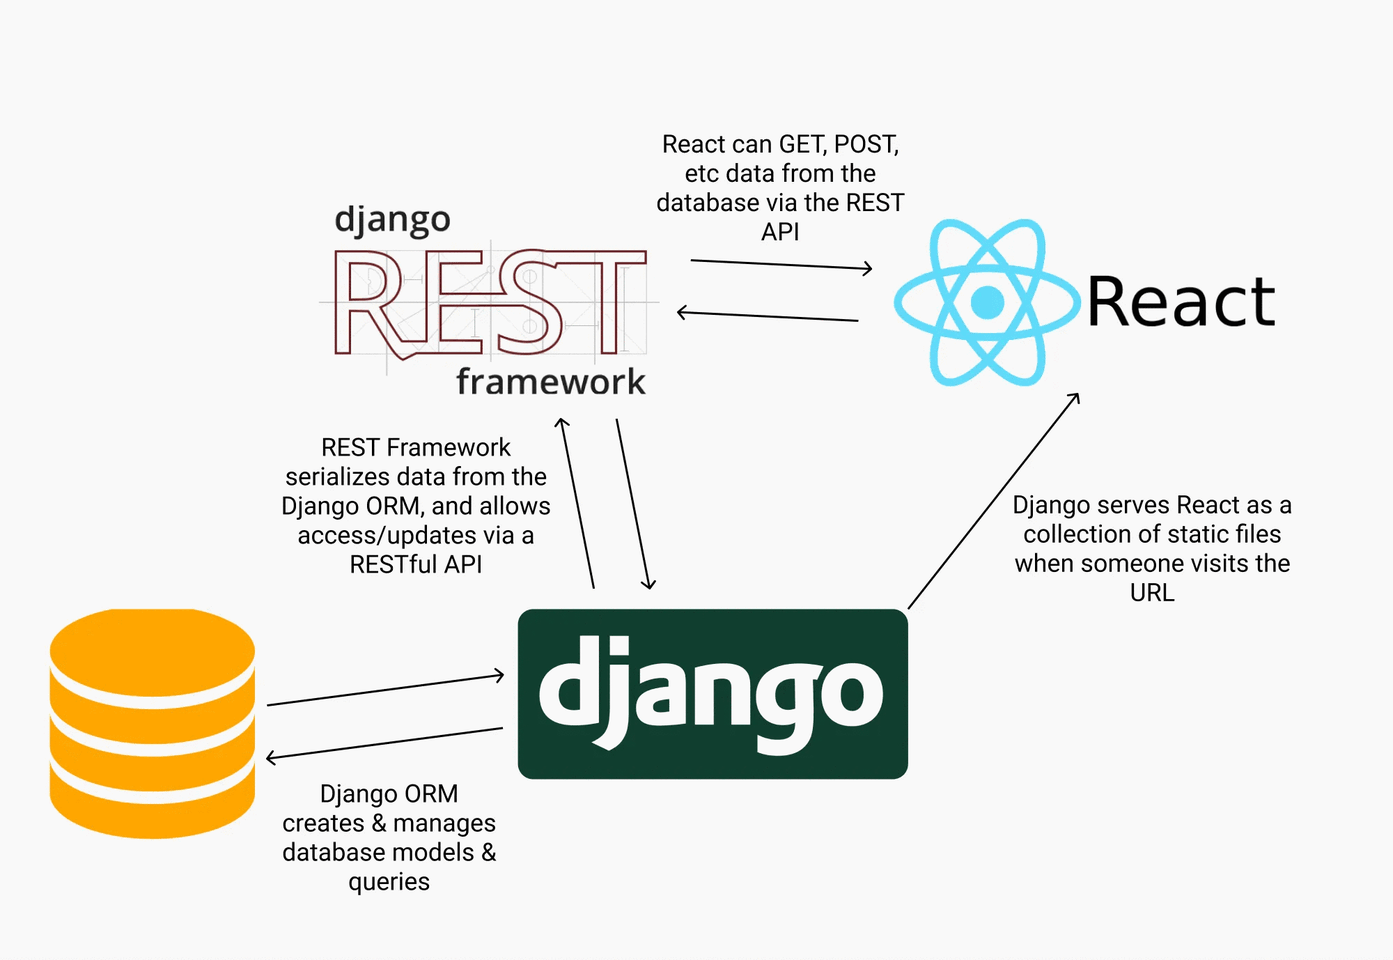
\includegraphics[width=0.9\textwidth]{techdesc}
	\centering
	\caption{Technical Architecture }
	\label{fig:techdesc}
 \cite{garner2021}
\end{figure}
\pagebreak


\subsection{Software Development Life Cycle}
We’ll adopt the Incremental Software Development Model, tackling requirements, research design, training, evaluation, and documentation in iterative cycles.

\begin{figure}[h]
	\includegraphics[width=\linewidth]{iteration}
	\centering
	\caption{Incremental model}
	\label{fig:iteration}
\end{figure}

In the first increment, we’ll analyze the project’s requirements, defining its scope, objectives, and constraints. For FOODFIND, this translates to pinpointing the system’s essential characteristics, such as restaurant menu and food data modeling, user profile, user reviews and recommendation. We’ll then embark on crucial research, gathering and examining data that aligns with these objectives. This entails investigating existing platforms providing similar services. We’ll gather the required data for the application using platforms providing dataset for testing purposes.

The second increment focuses on design, prototyping, and early testing. We’ll thoroughly plan the FOODFIND implementation, designing the system architecture, selecting suitable technologies, and developing streamlined prototypes to demonstrate core functionalities. This is followed by coding the core business logic and integrating them with the data sources. Rigorous tests will be conducted to validate initial functionality and identify potential areas for improvement. While initial deployment isn’t the primary focus here, preliminary feedback from the supervisor and the test results are valuable for ensuring the system is on track to meet the defined requirements.

The third increment revolves around refinement, integration, and enhanced testing. We’ll revisit and reiterate the requirements based on insights from testing, supervisor feedback, and evolving project goals. The research phase might involve acquiring additional data sets and investigating new research advancements. Taking into account the findings from the previous increment, we’ll optimize the system architecture, enhance the algorithms, and integrate feedback to improve the user interface. This phase also plays a more critical role in evaluation and improvement, quantifying the system’s effectiveness and identifying opportunities for further refinement.

The fourth increment marks the deployment, monitoring, and continuous improvement stage. The requirement analysis becomes an ongoing process, adapting to evolving business needs and incorporating user feedback. We’ll continuously benefit from new research findings allowing for ongoing adaptation. Finally, the evaluation and improvement become long-term endeavors, monitoring the system’s performance, gathering user feedback, and continuously improving the system.
\pagebreak

\subsection{Use Case Model}
The Use Case Model for the FoodFind project provides a structured representation of the interactions between users and the system. This section outlines the primary actors, their associated use cases, and the detailed scenarios that describe these interactions. The primary actors identified for the system are Users and Admins.

\subsubsection{Actors}
\begin{itemize}
    \item \textbf{User}: Represents the end-users of the FoodFind platform who interact with the system to search for, view, review and add restaurants as their favourite.
    \item \textbf{Admin}: Represents the system administrators who manage the restaurant data, user accounts, and ensure the overall system integrity.
\end{itemize}

\subsubsection{Use Cases for Users}

\paragraph{a. Login}
\begin{itemize}
    \item \textbf{Description}: The user logs into the FoodFind system.
    \item \textbf{Precondition}: The user must have an account with FoodFind.
    \item \textbf{Postcondition}: The user gains access to the system’s features.
\end{itemize}

\paragraph{b. Search Restaurant}
\begin{itemize}
    \item \textbf{Description}: Allows users to search for restaurants by name and location.
    \item \textbf{Precondition}: User is logged in or using the app without login (if allowed).
    \item \textbf{Postcondition}: Displays a list of restaurants matching the search criteria.
\end{itemize}

\paragraph{c. View Restaurant}
\begin{itemize}
    \item \textbf{Description}: Users can view details about different restaurants, including menus, prices, and available food items.
    \item \textbf{Precondition}: A restaurant has been selected from search results or another method of selection.
    \item \textbf{Postcondition}: Detailed information about the restaurant is displayed to the user.
\end{itemize}

\paragraph{d. Read Reviews}
\begin{itemize}
    \item \textbf{Description}: Users can read reviews provided by other users for various restaurants.
    \item \textbf{Precondition}: Reviews exist for a given restaurant.
    \item \textbf{Postcondition}: Reviews are displayed to help inform users’ choices.
\end{itemize}

\paragraph{e. Add Reviews}
\begin{itemize}
    \item \textbf{Description}: Users can provide reviews for restaurants they visit.
    \item \textbf{Precondition}: The user has visited a restaurant.
    \item \textbf{Postcondition}: The review is added to the restaurant’s profile.
\end{itemize}

\paragraph{f. Add Favorite Restaurant to User Profile}
\begin{itemize}
    \item \textbf{Description}: Users have the option to add their favorite restaurants to their profiles for easy access. This feature allows users to bookmark and revisit their preferred dining establishments without the need to search for them again.
    \item \textbf{Precondition}: The user is logged in.
    \item \textbf{Postcondition}: The restaurant is added to the user’s profile for future reference.
\end{itemize}

\subsubsection{Use Case Diagram for Users}
\begin{figure}[H]
    \centering
    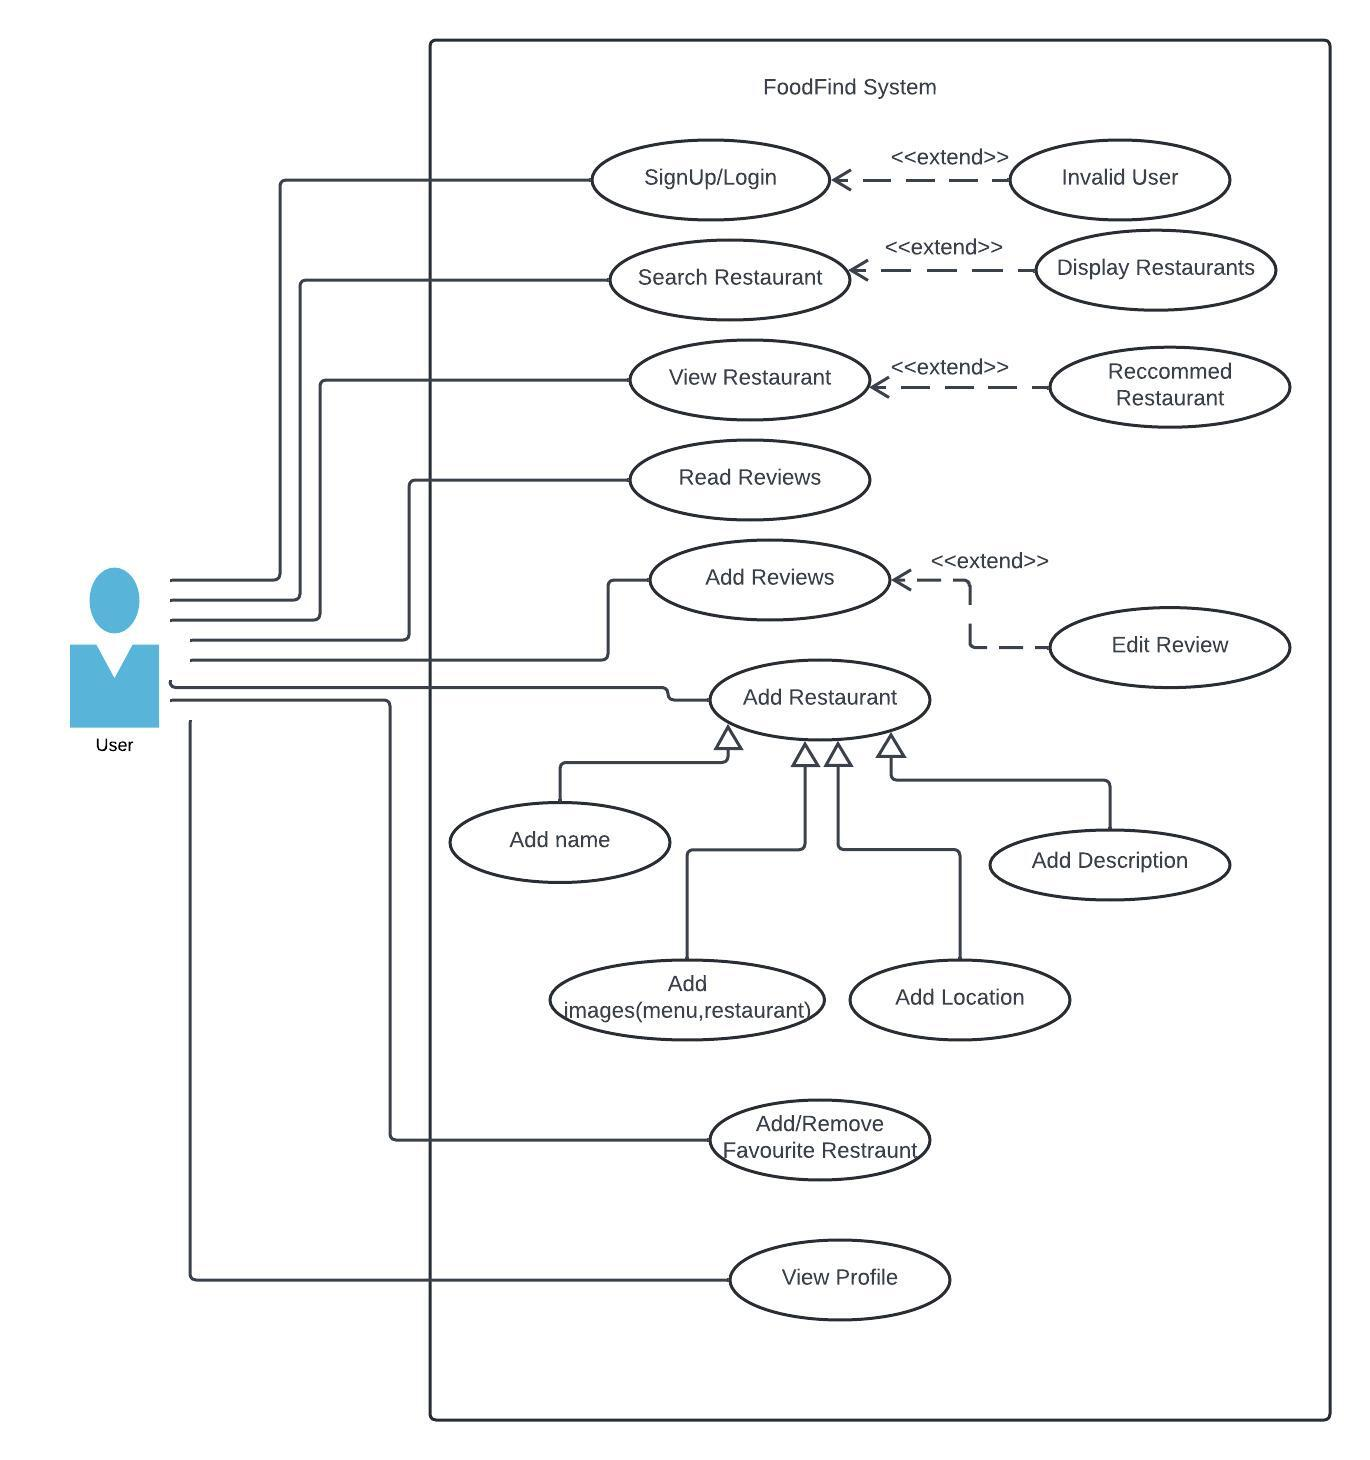
\includegraphics[width=\textwidth,height=\textheight,keepaspectratio]{images/usecaseUser.jpeg}
    \caption{Use Case Diagram for Users}
    \label{fig:usecaseUser1}
\end{figure}
\pagebreak
\subsubsection{Use Cases for Admin}

\paragraph{a. Login}
\begin{itemize}
    \item \textbf{Description}: Admin authenticates themselves to gain access to the system.
    \item \textbf{Precondition}: Admin must have valid credentials.
    \item \textbf{Postcondition}: Admin gains access to the system functionalities.
\end{itemize}

\paragraph{b. Add Restaurants}
\begin{itemize}
    \item \textbf{Description}: Admin adds new restaurant details into the system.
    \item \textbf{Precondition}: Admin must be logged in.
    \item \textbf{Postcondition}: New restaurant details are added into the system.
\end{itemize}

\paragraph{c. Verify Add Restaurant Request}
\begin{itemize}
    \item \textbf{Description}: Admin reviews and verifies requests for adding new restaurants.
    \item \textbf{Precondition}: There must be pending requests for adding restaurants.
    \item \textbf{Postcondition}: Requests are either approved or denied, updating the status of restaurant addition requests.
\end{itemize}

\paragraph{d. Update Restaurants}
\begin{itemize}
    \item \textbf{Description}: Admin modifies existing restaurant details in the system.
    \item \textbf{Precondition}: Restaurant details already exist in the system; admin must be logged in.
    \item \textbf{Postcondition}: Updated information of restaurants is saved in the system.
\end{itemize}

\paragraph{e. Delete Restaurants}
\begin{itemize}
    \item \textbf{Description}: Admin removes existing restaurant listings from FoodFind.
    \item \textbf{Precondition}: Restaurant listings exist; admin has authenticated access.
    \item \textbf{Postcondition}: Restaurant listings no longer appear on FoodFind.
\end{itemize}

\paragraph{f. Manage Users}
\begin{itemize}
    \item \textbf{Description}: Admin oversees user accounts, possibly editing or removing them.
    \item \textbf{Precondition}: Users have accounts within FoodFind; admin has authenticated access.
    \item \textbf{Postcondition}: User account data is updated or removed based on admin actions.
\end{itemize}


\subsubsection{Use Case Diagram for Admin}
\begin{figure}[H]
    \centering
    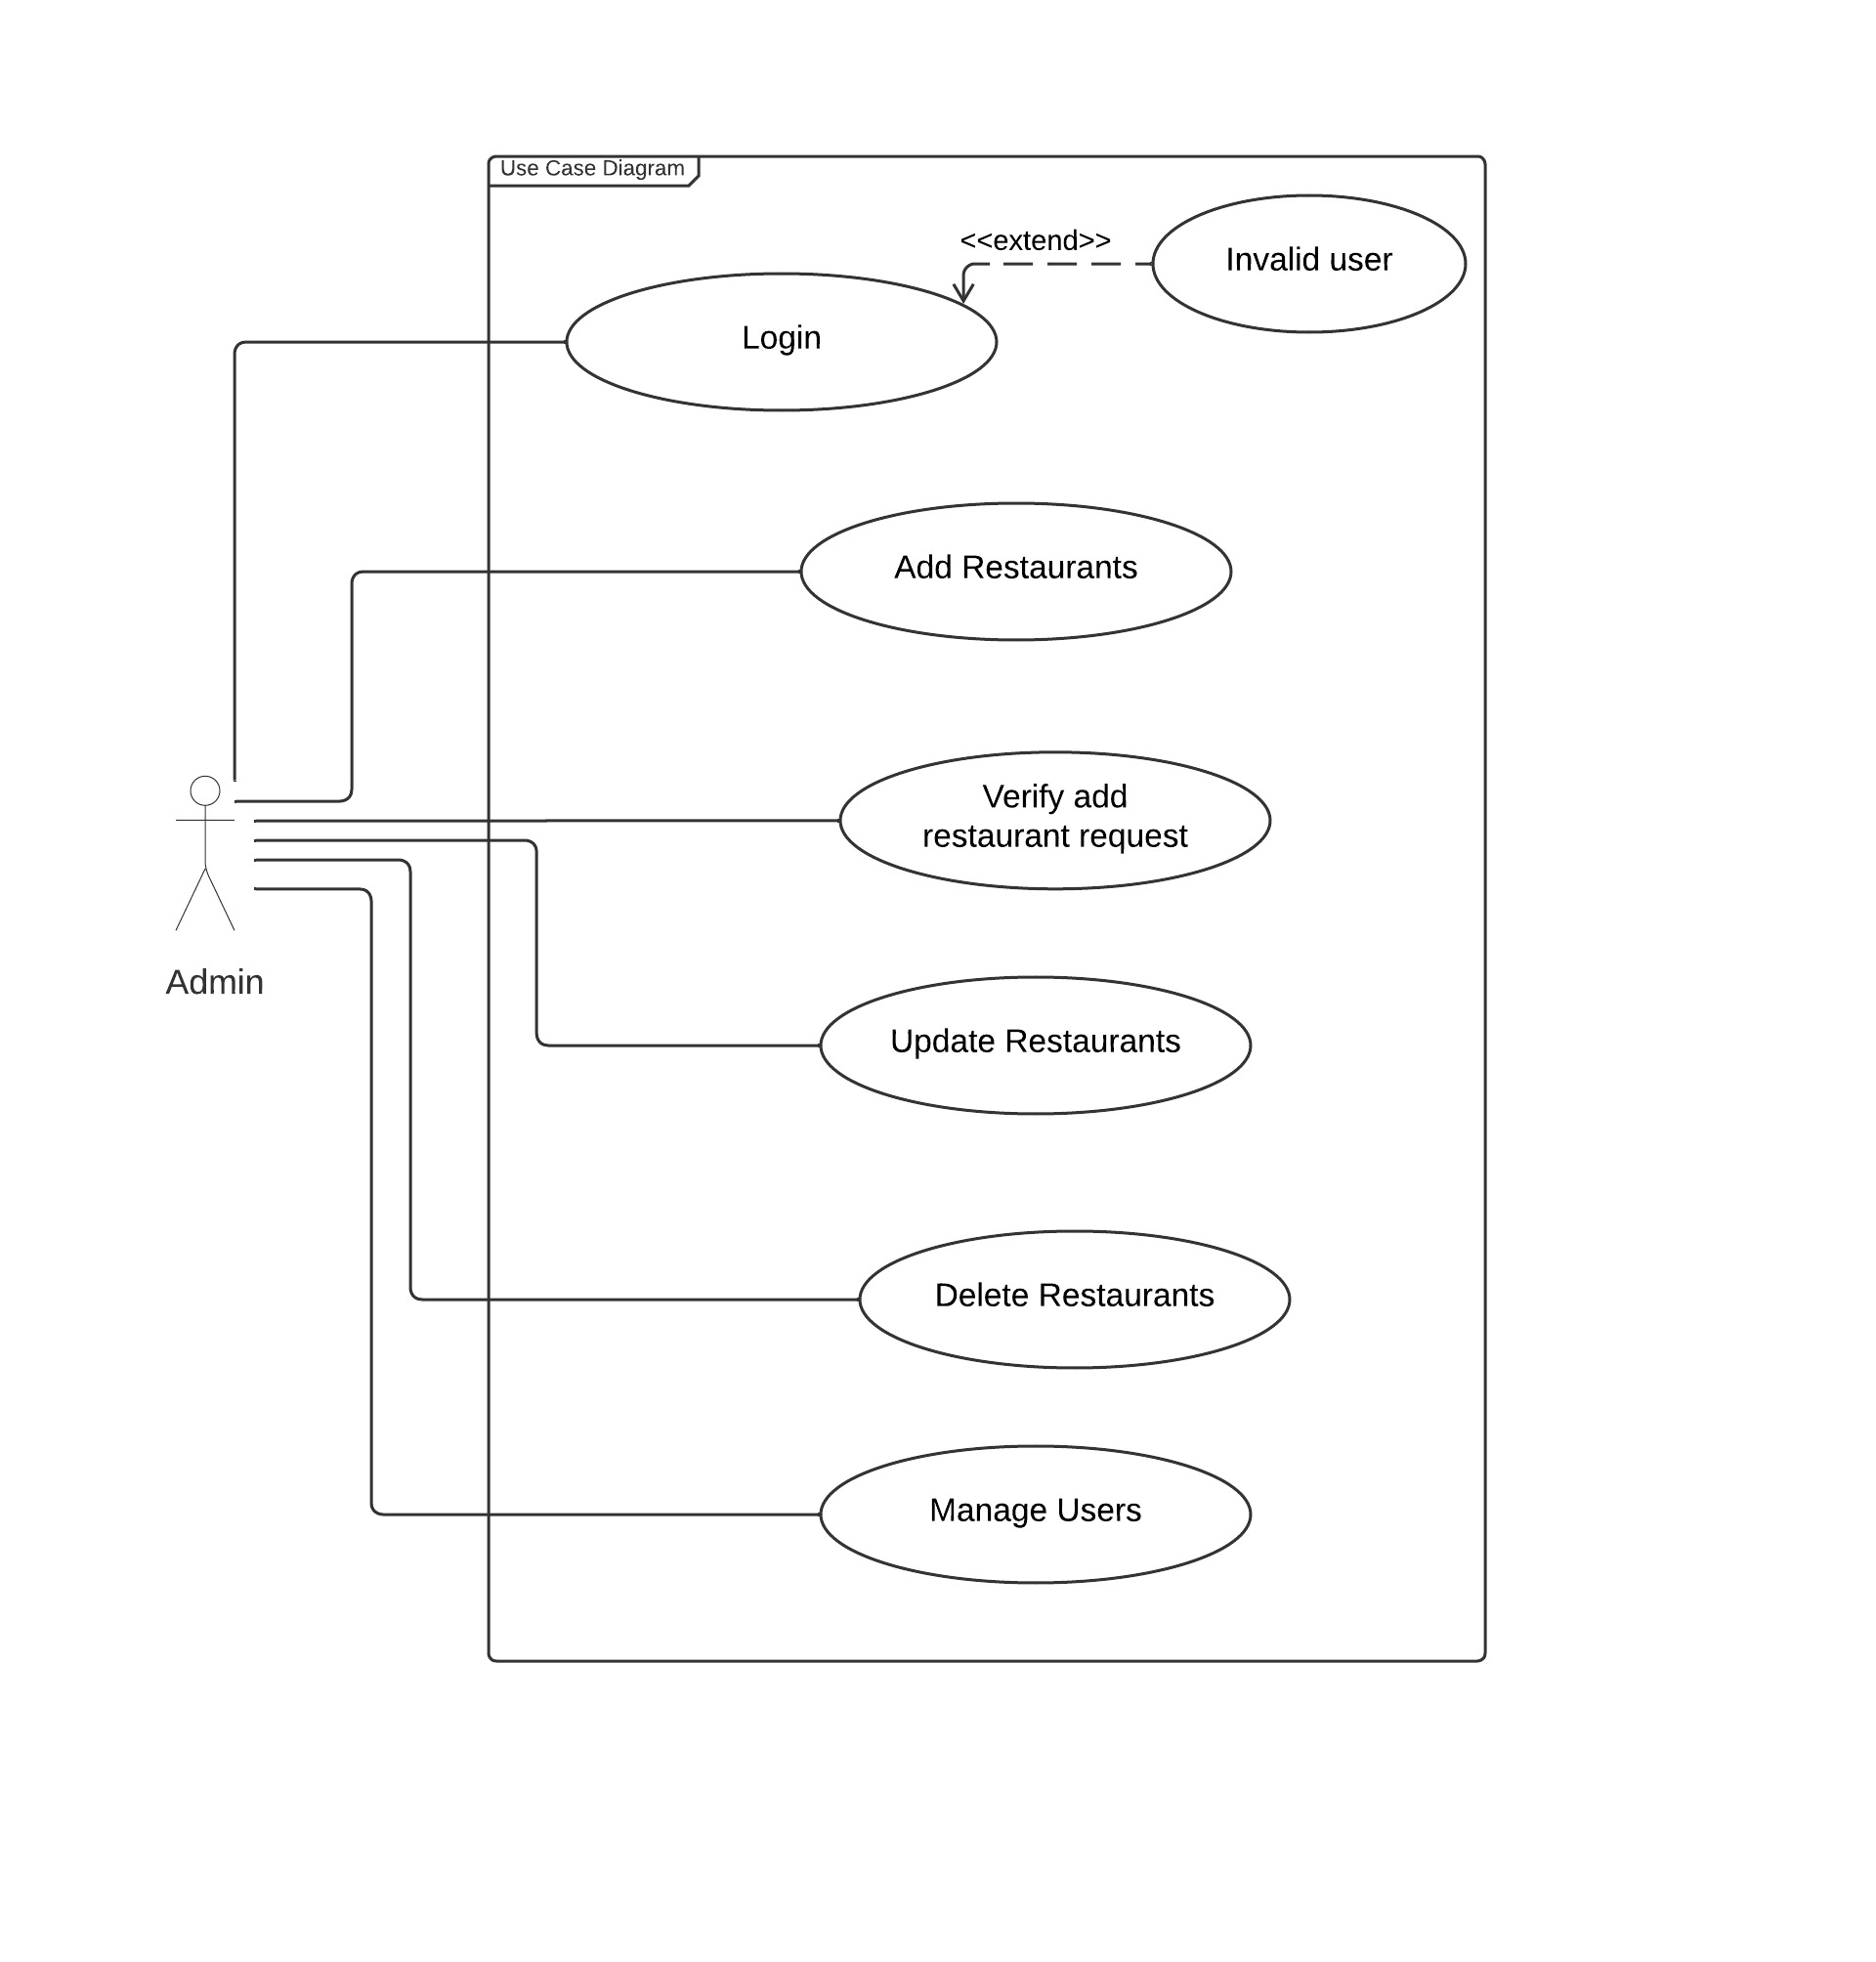
\includegraphics[width=\textwidth,height=\textheight,keepaspectratio]{images/useadmin.jpg}
    \caption{Use Case Diagram for Admin}
    \label{fig:useadmin}
\end{figure}
\pagebreak


% Garner, B. (2021, December 10)
%Source : https://bennettgarner.medium.com/react-on-django-getting-started-f30de8d23504


% \subsection{Class Diagram}
% The class diagram illustrates the structure of the FoodFind system by depicting its classes, attributes, methods, and the relationships between the classes. The main components of the diagram are as follows:

% \begin{itemize}
%     \item \textbf{Actor}
%     \begin{itemize}
%         \item \textbf{Attributes}: \texttt{id}, \texttt{name}, \texttt{password}
%         \item \textbf{Methods}: \texttt{login()}, \texttt{signup()}
%     \end{itemize}

%     \item \textbf{User (inherits from Actor)}
%     \begin{itemize}
%         \item \textbf{Methods}: \texttt{addRestaurant()}, \texttt{getMenus()}, \texttt{getReviews()}, \texttt{view\_history()}
%     \end{itemize}

%     \item \textbf{Admin (inherits from Actor)}
%     \begin{itemize}
%         \item \textbf{Methods}: \texttt{manage\_users()}, \texttt{verify\_restaurant()}
%     \end{itemize}

%     \item \textbf{Restaurant}
%     \begin{itemize}
%         \item \textbf{Attributes}: \texttt{restaurant\_id}, \texttt{restaurant\_name}, \texttt{verified}, \texttt{category}, \texttt{review\_id}
%         \item \textbf{Methods}: \texttt{addRestaurant()}, \texttt{viewDetails()}, \texttt{getMenus()}, \texttt{getReviews()}
%     \end{itemize}

%     \item \textbf{Menu}
%     \begin{itemize}
%         \item \textbf{Attributes}: \texttt{menuid}, \texttt{restaurant\_id}, \texttt{items}, \texttt{price}
%         \item \textbf{Methods}: \texttt{viewMenu()}, \texttt{editMenu()}
%     \end{itemize}

%     \item \textbf{Review}
%     \begin{itemize}
%         \item \textbf{Attributes}: \texttt{review\_id}, \texttt{id}, \texttt{restaurant\_id}, \texttt{rating}, \texttt{comment}
%         \item \textbf{Methods}: \texttt{updateReview()}
%     \end{itemize}

%     \item \textbf{Relationships}
%     \begin{itemize}
%         \item \textbf{Inheritance}: User and Admin inherit from Actor.
%         \item \textbf{Associations}: Users and Admins interact with Restaurants and Menus.
%     \end{itemize}
% \end{itemize}

% This diagram concisely represents FoodFind's system components and their interactions.
% \begin{figure}[H]
%     \centering
%     \rotatebox{90}{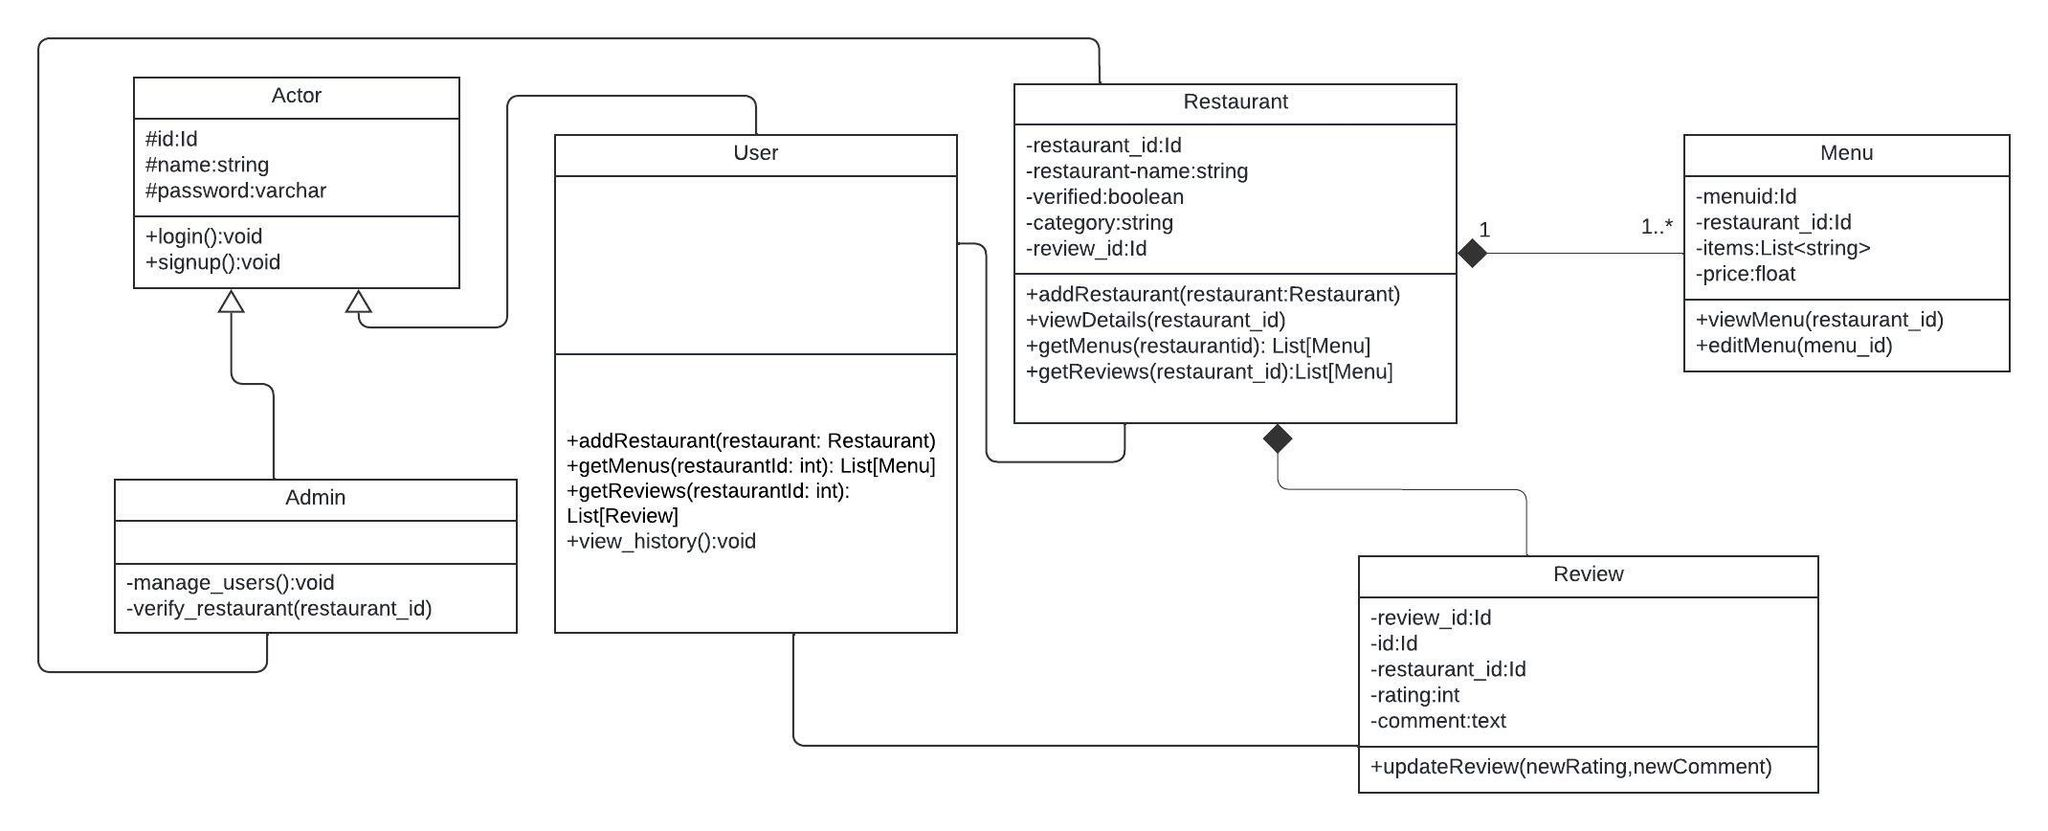
\includegraphics[width=0.9\textheight]{classdiag}}
%     \caption{Class Diagram}
%     \label{fig:classdiag}
% \end{figure}



\subsection{Sequence Diagram}
A sequence diagram is a graphical representation that illustrates the interactions between objects or components within a system in a chronological order, aiding developers in understanding system behavior, identifying patterns, and validating design decisions.

The user interacts with the FoodFind System to perform various actions, such as logging in, searching for restaurants, viewing menus, adding reviews, and sharing restaurant locations.

The system communicates with the Database to check user details during login, query restaurant data, and update information based on user reviews or newly added restaurants.

\begin{figure}[H]
    \centering
    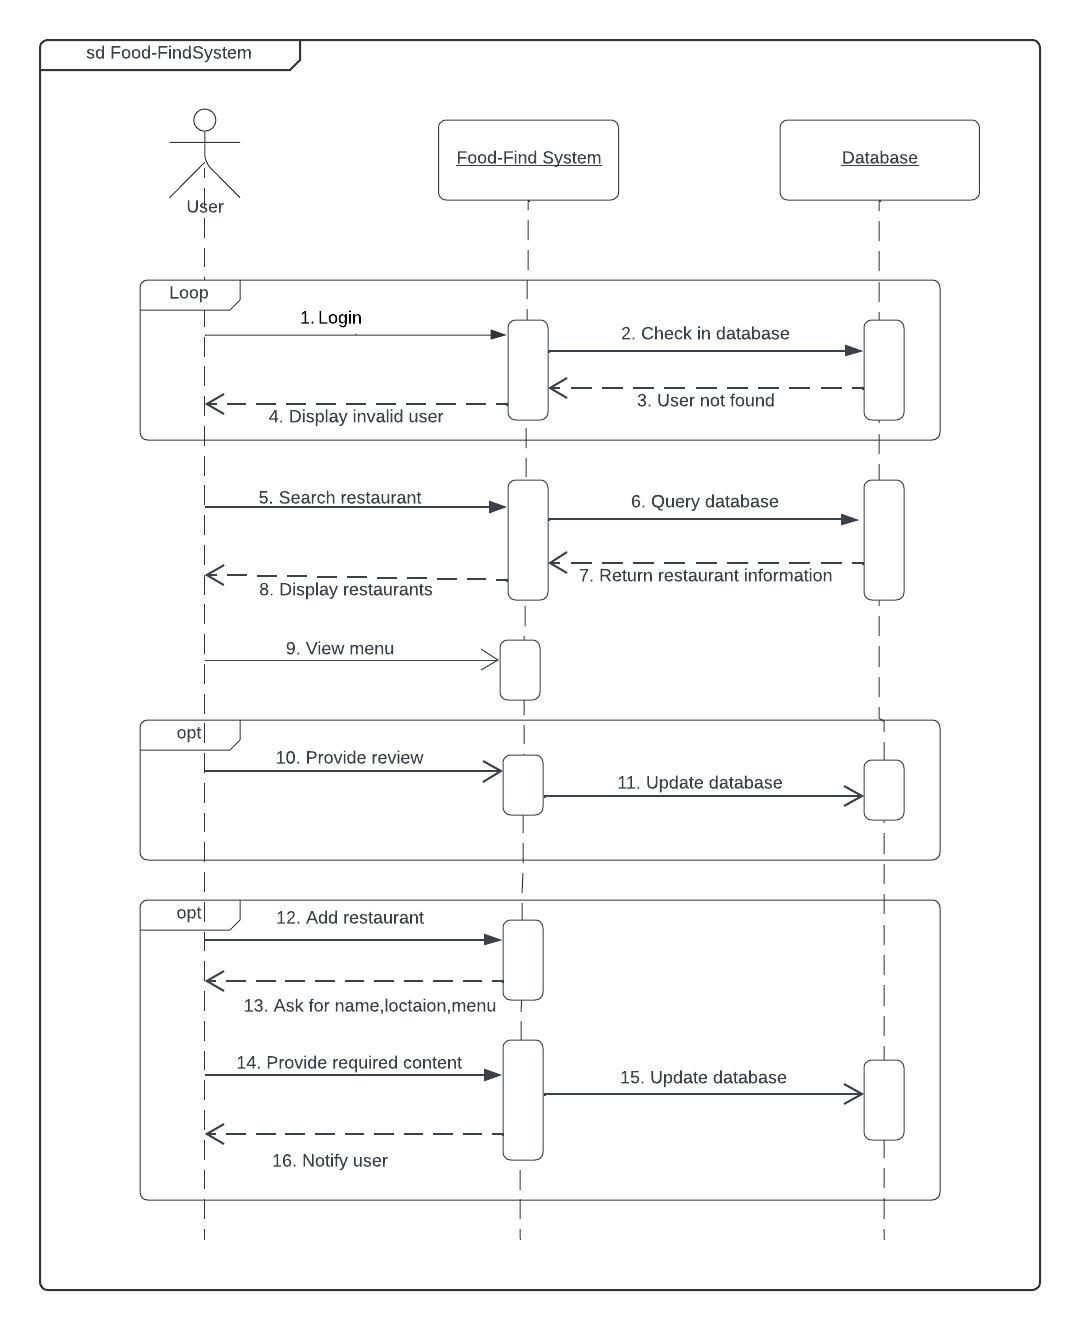
\includegraphics[width=\textwidth, height=\textheight, keepaspectratio]{images/sequence.jpg}
    \caption{Sequence Diagram}
    \label{fig:sequencediag}
\end{figure}


\pagebreak

\subsection{Database Diagram}

The diagram is data model for FoodFind database. It outlines the structure and relationships between different entities in the  database. Here's a brief explanation of each entity and its attributes

\subsubsection{Entities and Their Attributes}

\begin{itemize}
    \item \textbf{Customers}
    \begin{itemize}
        \item \textbf{customer\_id}: Primary Key, INT, NOT NULL
        \item \textbf{username}: VARCHAR(150), NOT NULL
        \item \textbf{email}: VARCHAR(254), UNIQUE, NOT NULL
        \item \textbf{google\_id}: VARCHAR(255), UNIQUE, NOT NULL
        \item \textbf{profile\_picture}: VARCHAR(200)
        \item \textbf{favourite\_restaurants}: Many-to-Many relationship with \textbf{Restaurant}, NOT NULL
    \end{itemize}

    \item \textbf{Review}
    \begin{itemize}
        \item \textbf{id}: Primary Key, INT, NOT NULL
        \item \textbf{user\_id}: Foreign Key referencing \textbf{customer\_id}, INT, NOT NULL
        \item \textbf{restaurant\_id}: Foreign Key referencing \textbf{restaurant\_id}, INT, NOT NULL
        \item \textbf{rating}: INT, NOT NULL
        \item \textbf{review\_text}: TEXT
        \item \textbf{created\_at}: DATETIME, NOT NULL
        \item \textbf{updated\_at}: DATETIME, NOT NULL
    \end{itemize}

    \item \textbf{Restaurant}
    \begin{itemize}
        \item \textbf{restaurant\_id}: Primary Key, INT, NOT NULL
        \item \textbf{name}: VARCHAR(255), NOT NULL
        \item \textbf{location}: VARCHAR(255), NOT NULL
        \item \textbf{price}: VARCHAR(100), NOT NULL
        \item \textbf{opening\_hours}: VARCHAR(100), NOT NULL
        \item \textbf{description}: TEXT, NOT NULL
        \item \textbf{map\_url}: VARCHAR(500), NOT NULL
    \end{itemize}

    \item \textbf{Menu}
    \begin{itemize}
        \item \textbf{id}: Primary Key, INT, NOT NULL
        \item \textbf{restaurant\_id}: Foreign Key referencing \textbf{restaurant\_id}, INT, NOT NULL
        \item \textbf{name}: VARCHAR(255), NOT NULL
        \item \textbf{price}: DECIMAL(10, 2), NOT NULL
        \item \textbf{category}: VARCHAR(20), NOT NULL
    \end{itemize}

    \item \textbf{Tags}
    \begin{itemize}
        \item \textbf{id}: Primary Key, INT, NOT NULL
        \item \textbf{name}: VARCHAR(50), UNIQUE, NOT NULL
    \end{itemize}

    \item \textbf{TopRestaurant}
    \begin{itemize}
        \item \textbf{id}: Primary Key, INT, NOT NULL
        \item \textbf{restaurant\_id}: Foreign Key referencing \textbf{restaurant\_id}, INT
        \item \textbf{ranking}: INT, UNIQUE, NOT NULL
    \end{itemize}

    \item \textbf{RestaurantImage}
    \begin{itemize}
        \item \textbf{id}: Primary Key, INT, NOT NULL
        \item \textbf{restaurant\_id}: Foreign Key referencing \textbf{restaurant\_id}, INT, NOT NULL
        \item \textbf{image}: VARCHAR(100), NOT NULL
    \end{itemize}
\end{itemize}
\begin{figure}[H]
    \centering
    \rotatebox{90}{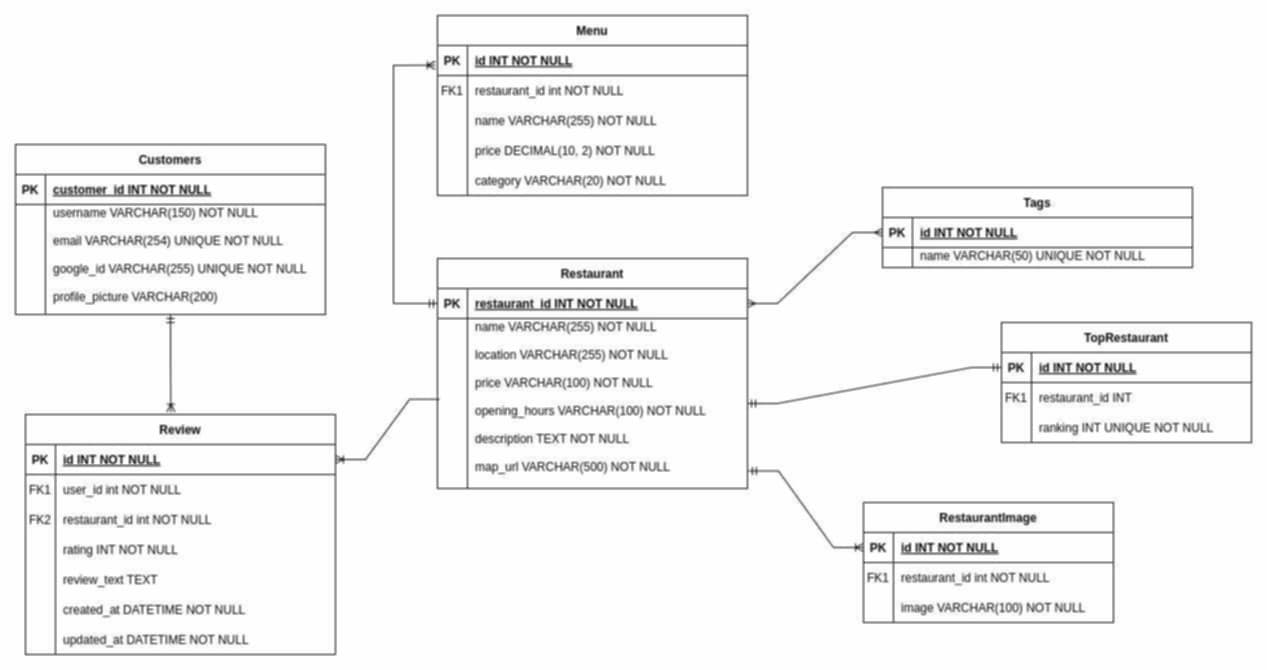
\includegraphics[width=0.9\textheight]{images/databaseD.jpg}}
    \caption{Database Diagram}
    \label{databaseD}
\end{figure}
\subsubsection{Relationships}

\begin{itemize}
    \item \textbf{Customers to Review}: One customer can write multiple reviews (\textbf{user\_id} in Review references \textbf{customer\_id} in Customers).
    \item \textbf{Restaurant to Review}: One restaurant can have multiple reviews (\textbf{restaurant\_id} in Review references \textbf{restaurant\_id} in Restaurant).
    \item \textbf{Restaurant to Menu}: One restaurant can have multiple menu items (\textbf{restaurant\_id} in Menu references \textbf{restaurant\_id} in Restaurant).
    \item \textbf{Restaurant to Tags}: Many-to-many relationship implied (not explicitly shown but generally implemented with a join table).
    \item \textbf{Restaurant to TopRestaurant}: One restaurant can be listed as a top restaurant with a unique ranking (\textbf{restaurant\_id} in TopRestaurant references \textbf{restaurant\_id} in Restaurant).
    \item \textbf{Restaurant to RestaurantImage}: One restaurant can have multiple images (\textbf{restaurant\_id} in RestaurantImage references \textbf{restaurant\_id} in Restaurant).
\end{itemize}

This ERD represents the database schema for managing customers, restaurants, reviews, menus, tags, top restaurant rankings, and restaurant images.




\pagebreak

\subsection{Activity Diagram}
An activity diagram for FoodFind represents the user journey and interactions within the restaurant recommendation application. It shows the sequence of activities, such as signing up, logging in, searching, filtering, and reviewing restaurants, as well as decisions like whether to register or add a new restaurant. This helps in understanding how users navigate through the application and the flow of various functionalities. 

\subsubsection{Overall User Activity}
The following  activity diagram illustrates the user flow within the FoodFind System:
\begin{enumerate}
    \item \textbf{SignUp/Login}: Users start by signing up or logging in if already registered.
    \item \textbf{Registration}: New users enter details to create an account.
    \item \textbf{Login Validation}: Credentials are validated; successful login leads to viewing restaurants.
    \item \textbf{View/Search Restaurants}: Users can view all restaurants or search for specific ones.
    \item \textbf{Filer Restaurants}: Users filter search results by food type or tags.
    \item \textbf{View Details/Results}: Users view detailed information about selected restaurants.
    \item \textbf{Provide Review}: Users can leave reviews for restaurants.
    \item \textbf{Request to Add Restaurant}: If a restaurant is not listed, users can request to add it by providing details.
\end{enumerate}
The diagram effectively maps the decision points and actions a user takes within the FoodFind app.
\begin{figure}[H]
	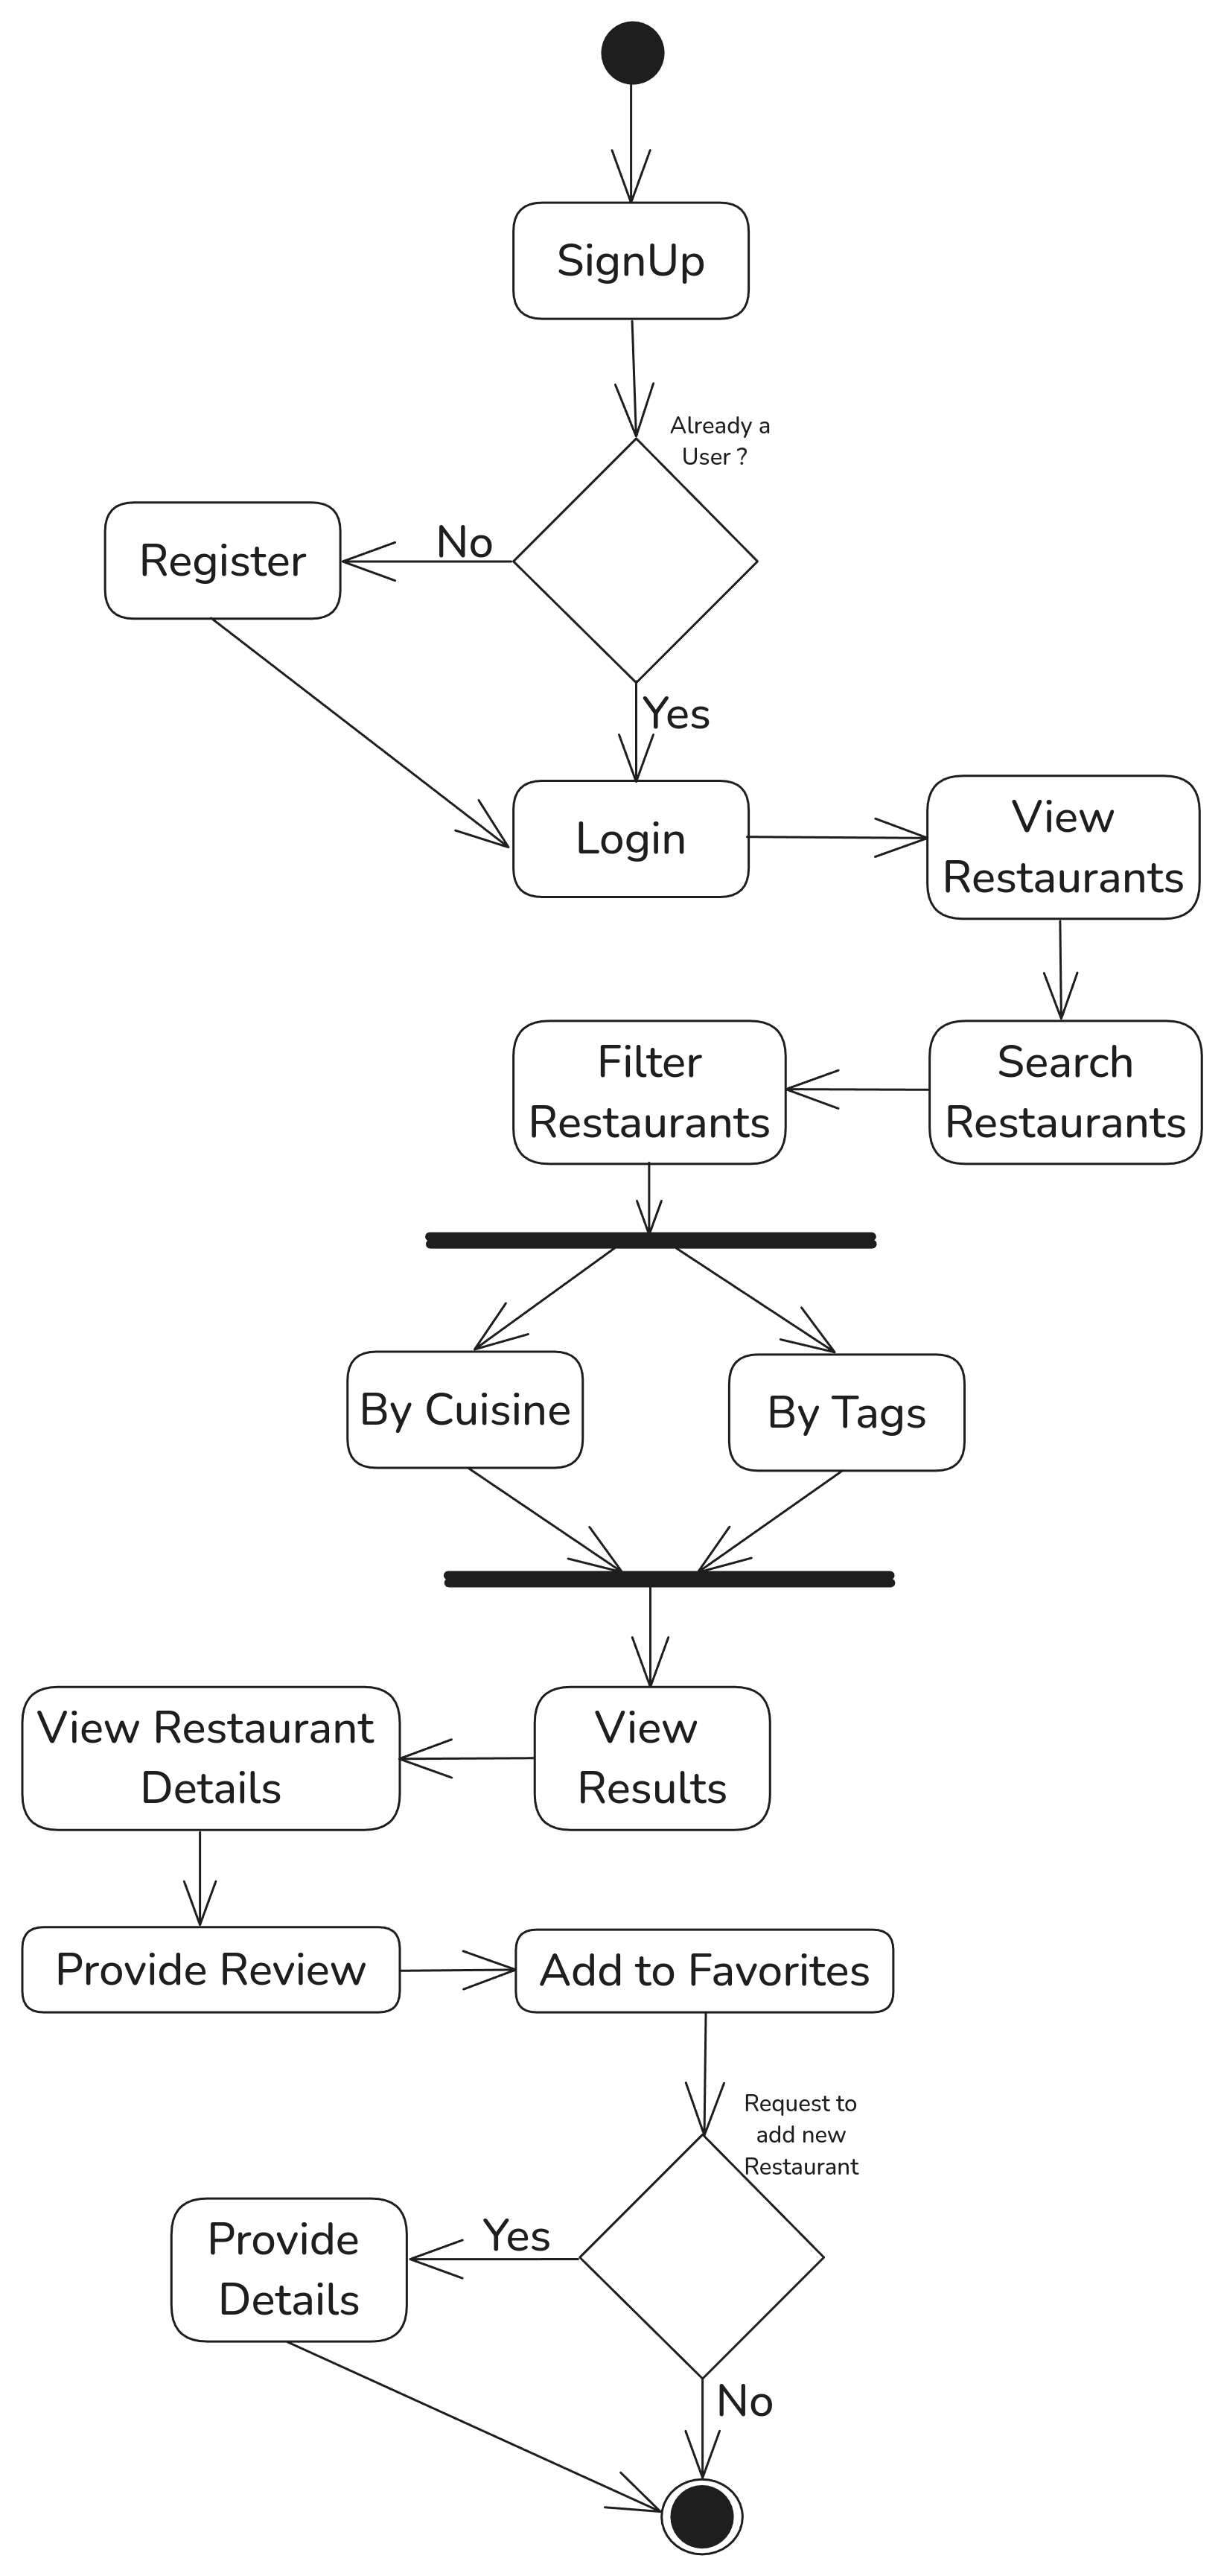
\includegraphics[width=0.8\textwidth, height=\textheight, keepaspectratio]{images/useractivity.png}
	\centering
	\caption{Activity Diagram for User}
	\label{fig:activity}
\end{figure}
\pagebreak

\subsubsection{Providing Review}
Figure \ref{fig:review} illustrates the user’s process of selecting a restaurant, writing a review, and the subsequent update to the restaurant’s profile with the new review.
\begin{figure}[H]
    \centering
    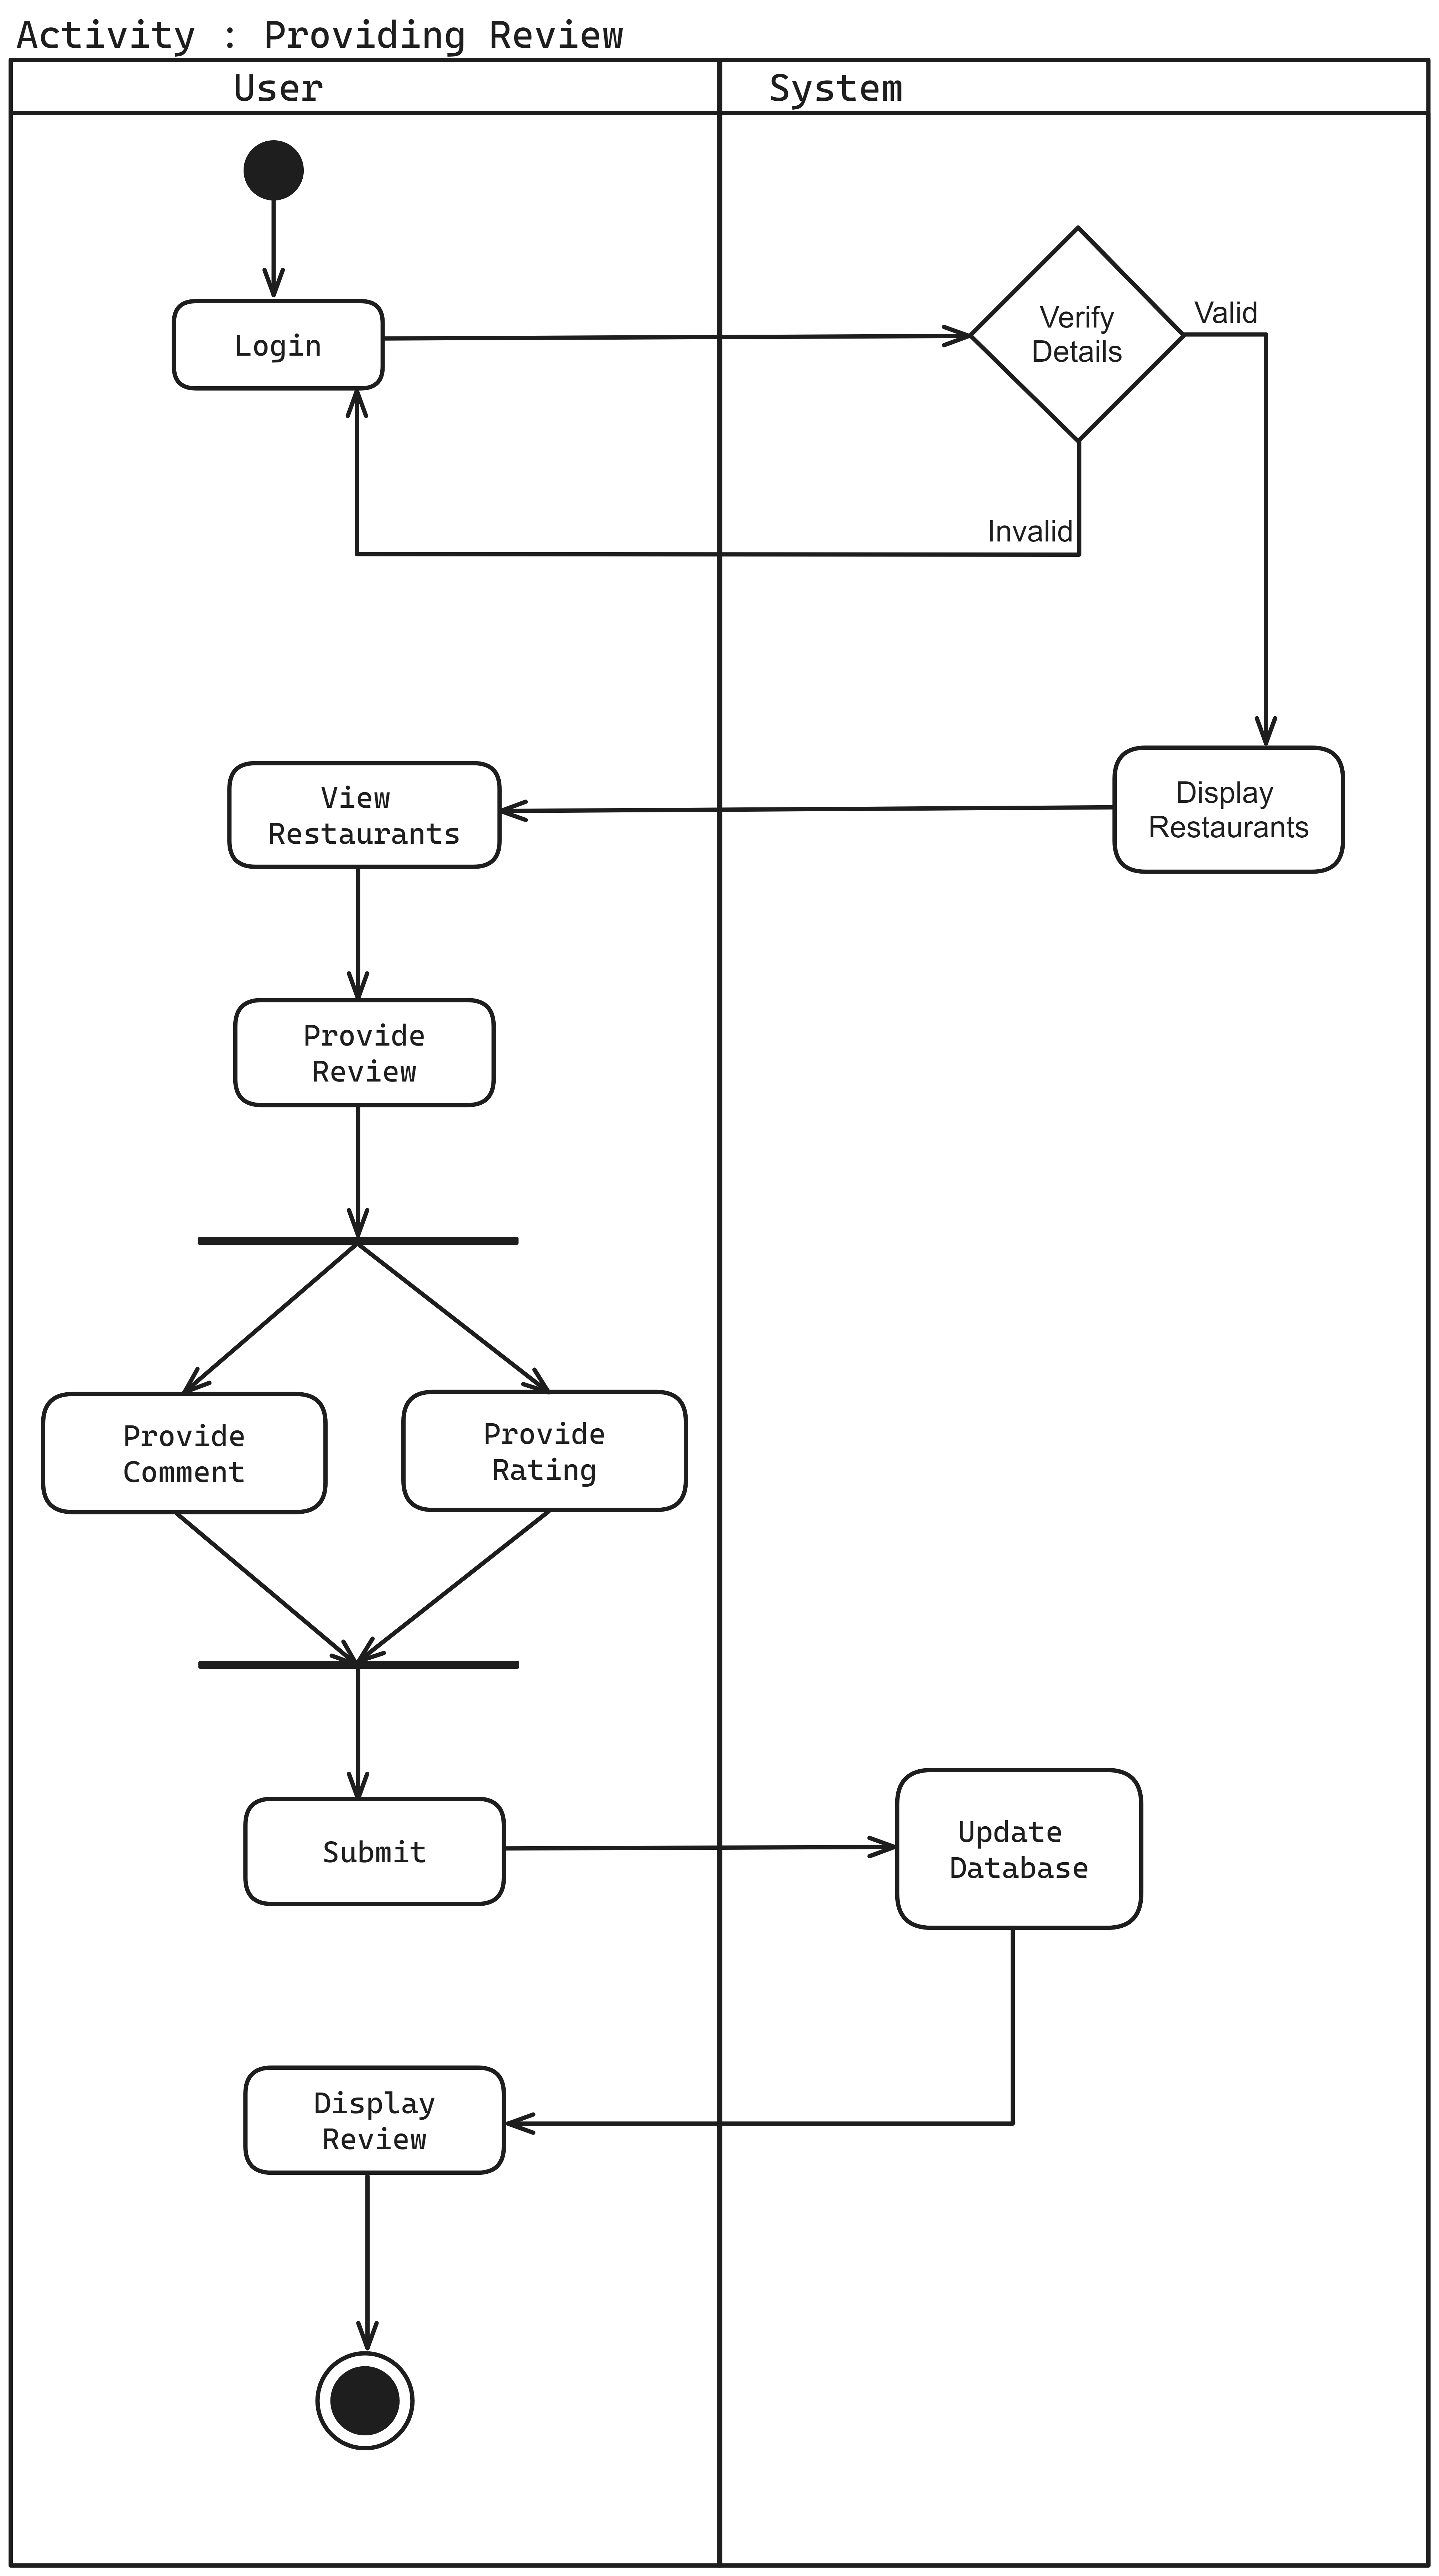
\includegraphics[width=0.8\textwidth, height=\textheight, keepaspectratio]{images/review.png}
    \caption{Activity Diagram for Providing ReviEW}
    \label{fig:review}
\end{figure}
\pagebreak


\subsubsection{Adding a Restaurant}
Figure \ref{fig:addres} illustrates the user’s request to add a new restaurant and the subsequent approval process handled by an admin, ensuring quality control before the listing goes live on FoodFind.
\vspace{2mm}
\begin{figure}[h]
	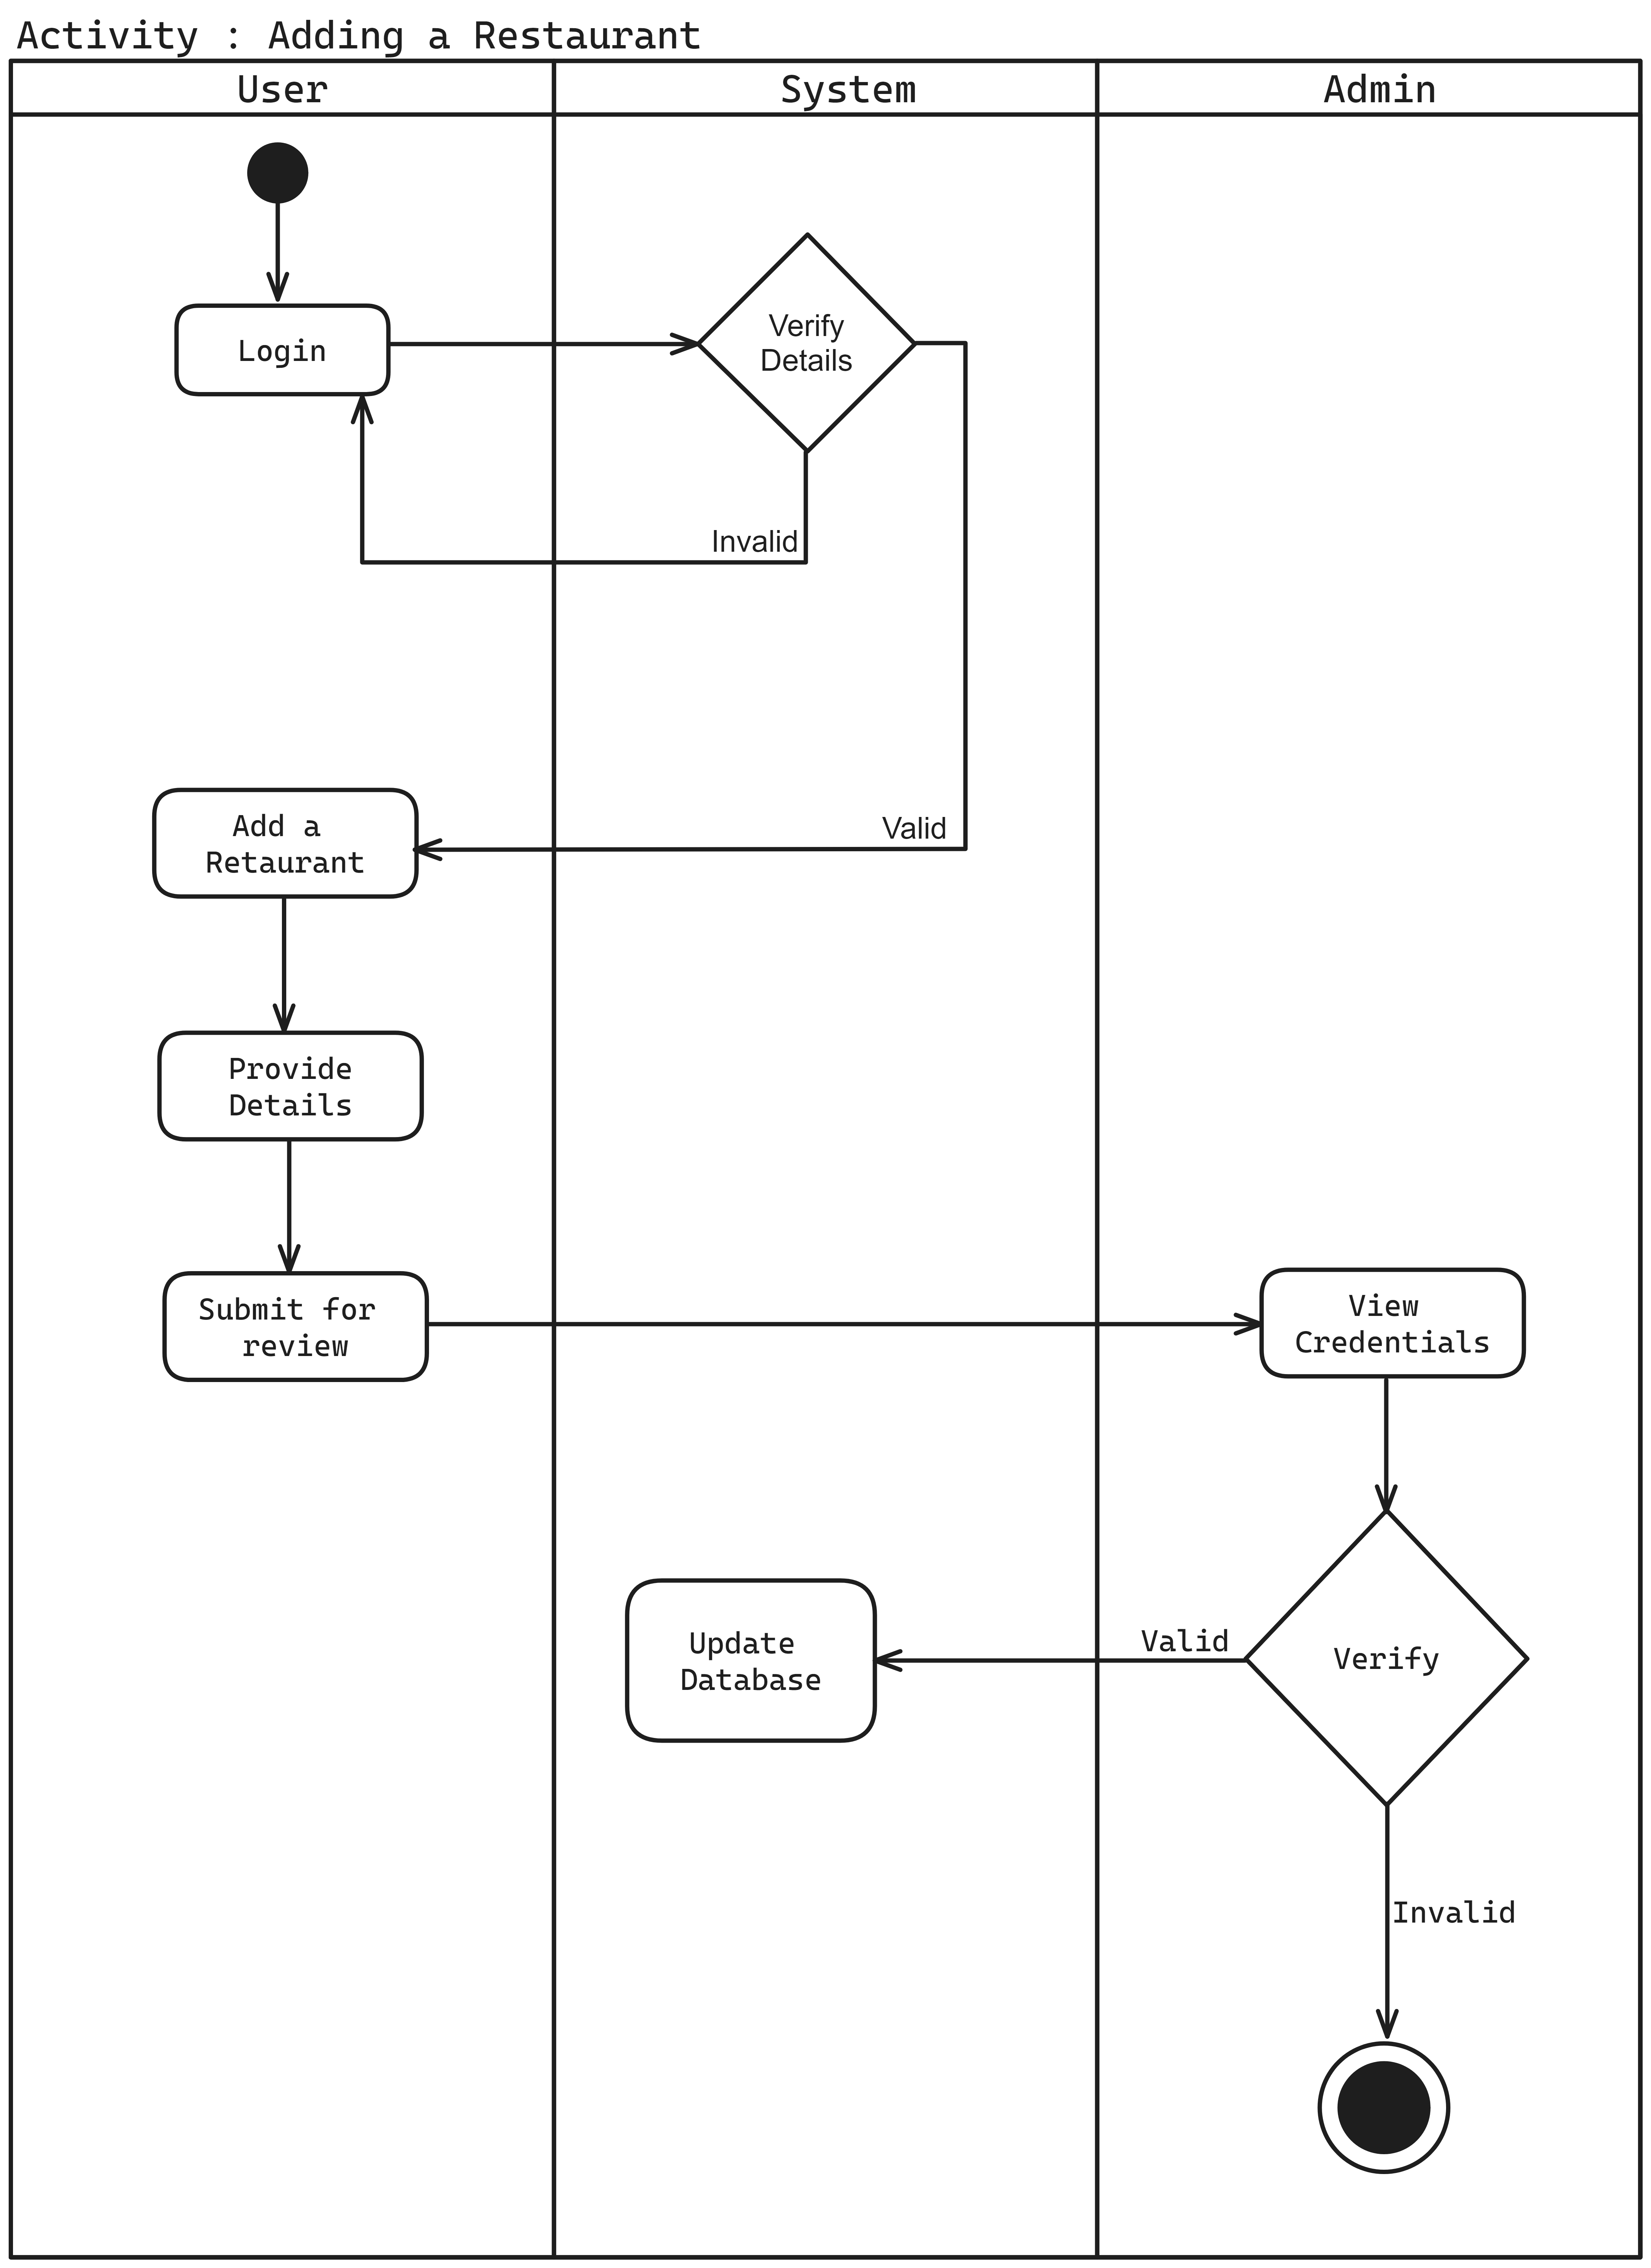
\includegraphics[width=0.7\textwidth]{images/adding.png}
	\centering
	\caption{Activity Diagram for Adding Restaurants}
	\label{fig:addres}
\end{figure}
\pagebreak


\subsection{System Flow}
In context of FoodFind, below Figure \ref{fig:system flow} illustrates a streamlined web development architecture where TypeScript is the core language for the frontend, transpiled by Vite and styled with Tailwind CSS and Daisy UI for a responsive design. 

The frontend communicates with the backend via a REST API, which is powered by Django Restful API, utilizing Django ORM for object-relational mapping and SQLite for database management. This setup ensures a robust, scalable, and maintainable web application framework.
\vspace{2mm}

\begin{figure}[H]
    \centering
    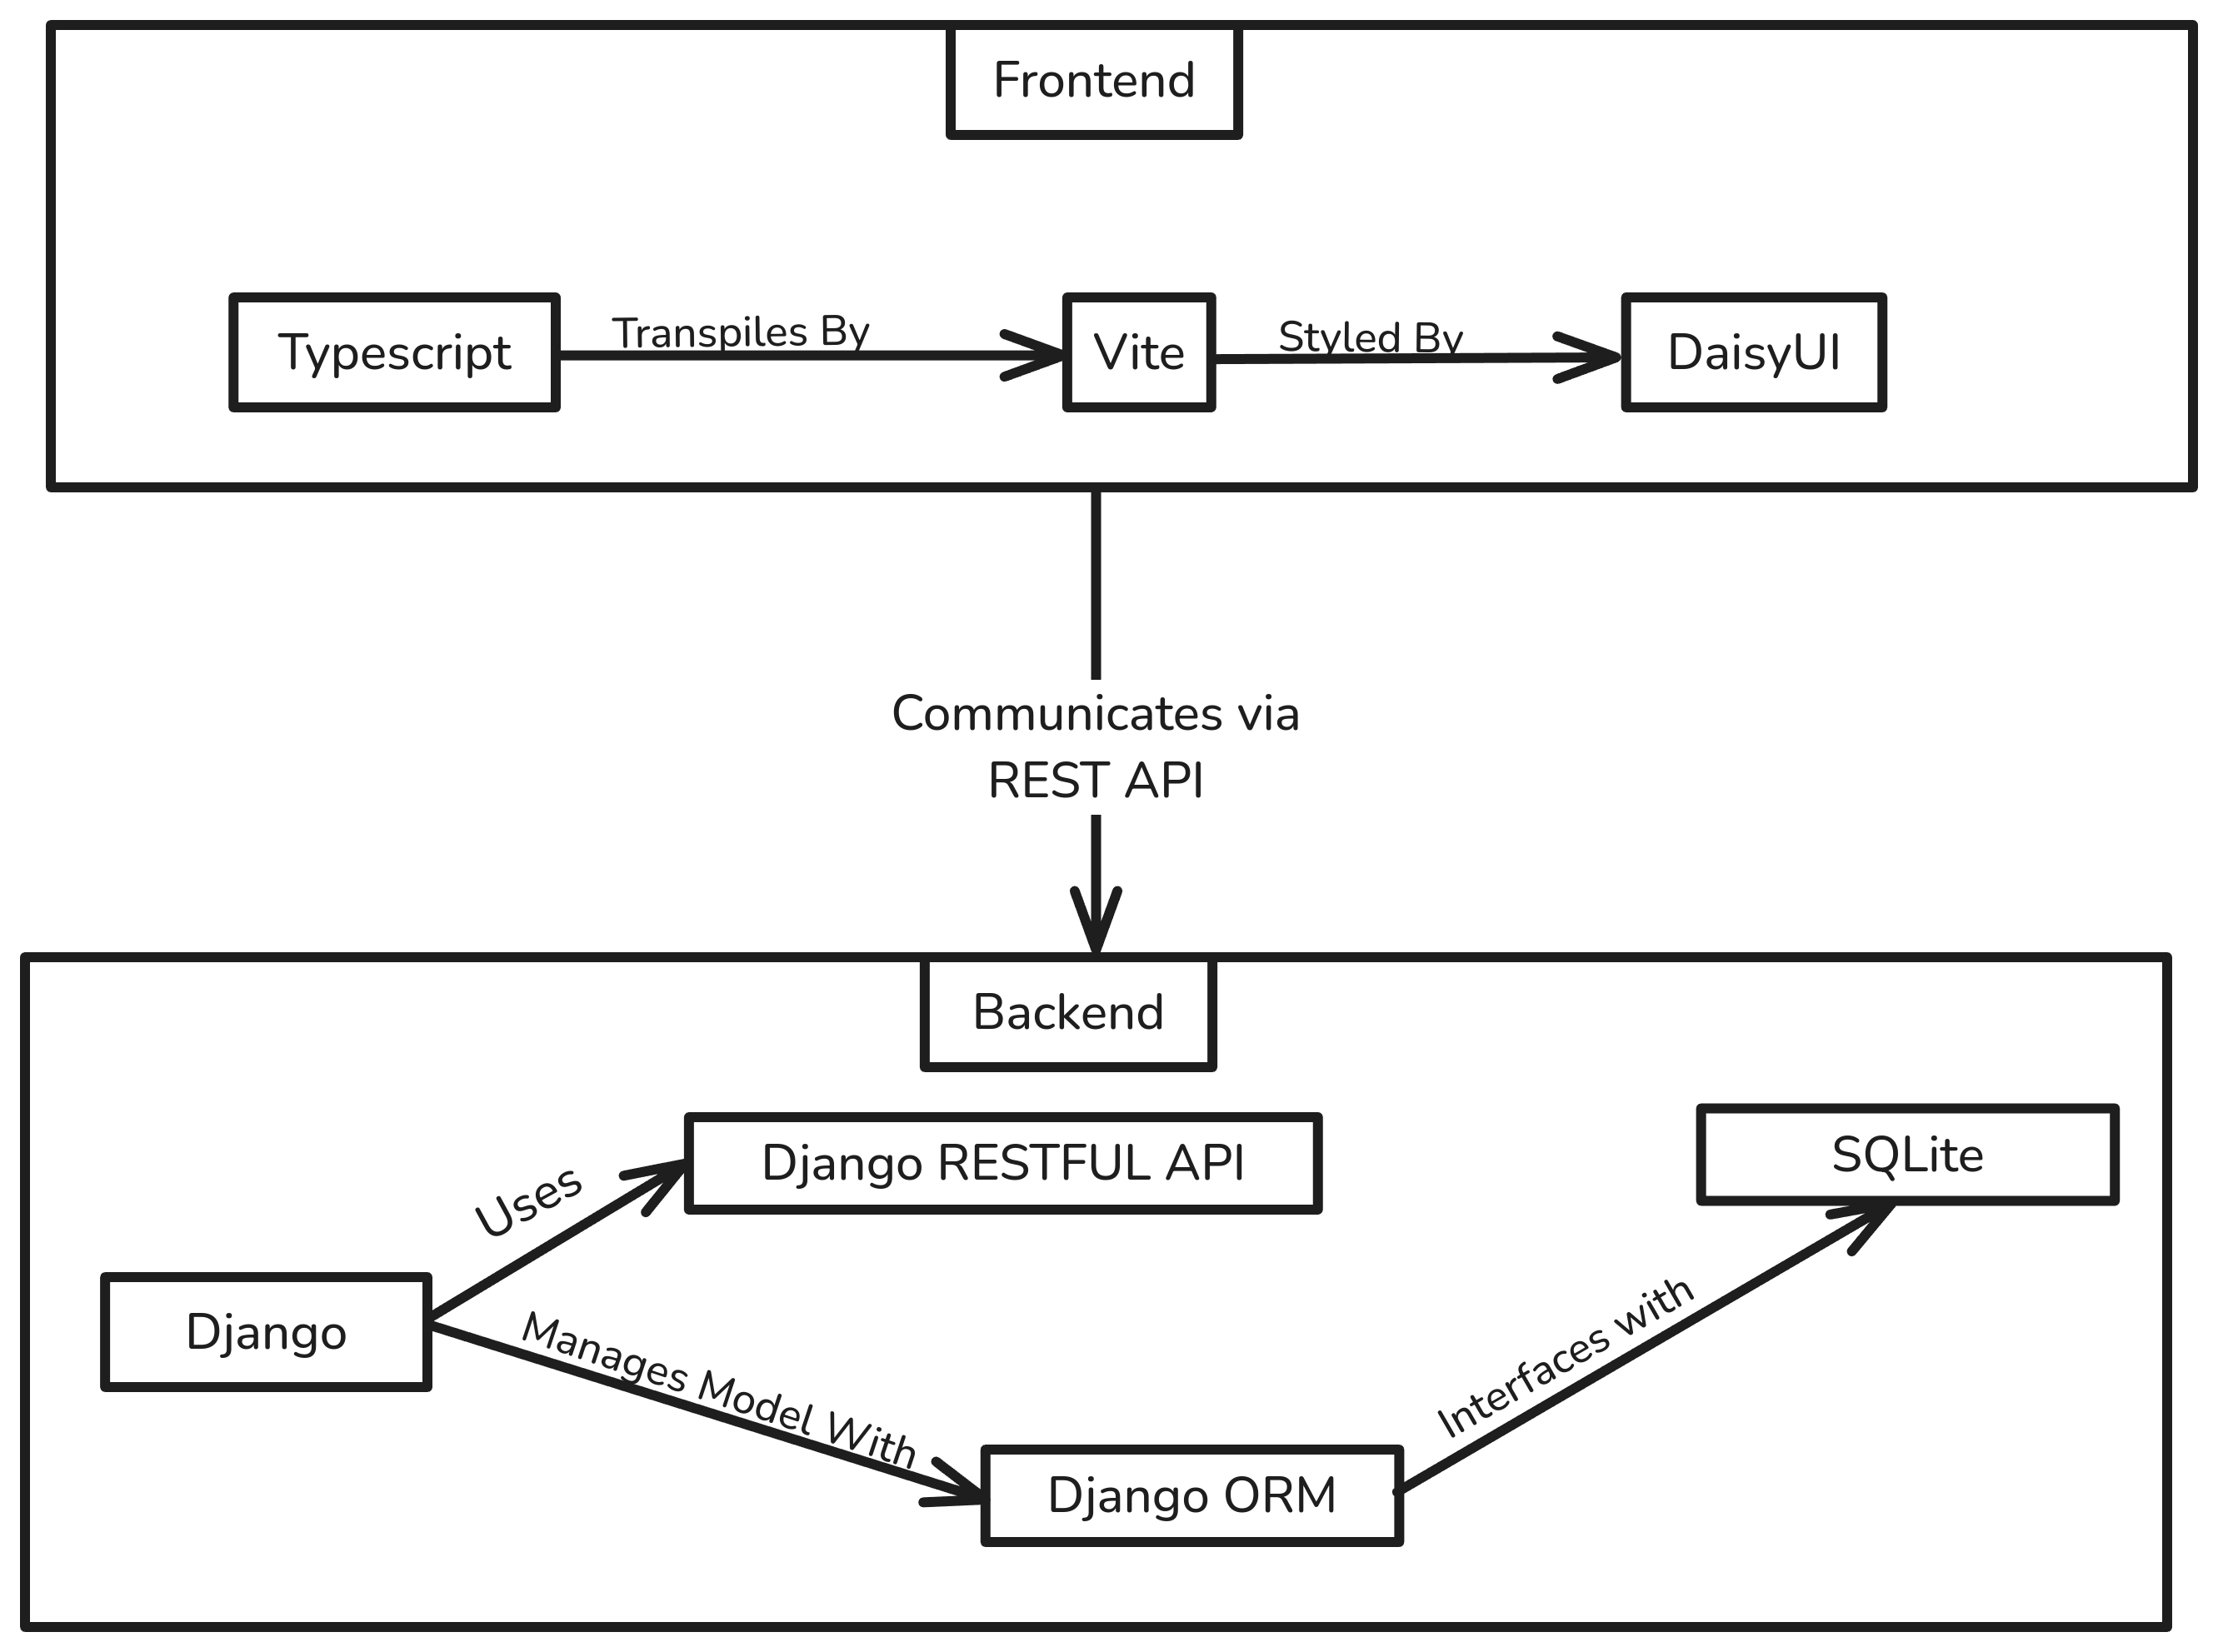
\includegraphics[width=\textwidth,height=\textheight,keepaspectratio]{system flow}
    \caption{System Flow Diagram}
    \label{fig:system fLow}
\end{figure}
\pagebreak


\subsection{Component Diagram}

The component diagram illustrates the architectural structure of the FoodFind system by showing the components and their relationships. Here's a brief explanation of the key components and their interactions:

\subsubsection*{Components}
\begin{itemize}
    \item \textbf{CuisineModel, RestaurantModel, ReviewsModel, AdminModel}
    \begin{itemize}
        \item These are the core models representing different entities in the FoodFind system.
        \item They handle the data and logic related to cuisines, restaurants, reviews, and admin functionalities, respectively.
    \end{itemize}

    \item \textbf{ORM (Object-Relational Mapping)}
    \begin{itemize}
        \item This component manages database interactions.
        \item It converts data between incompatible type systems in object-oriented programming and relational databases.
    \end{itemize}

    \item \textbf{Views}
    \begin{itemize}
        \item This component is responsible for rendering the user interface elements.
        \item It interacts with the models to fetch data and present it to the users.
    \end{itemize}

    \item \textbf{ApiEndpoints}
    \begin{itemize}
        \item These endpoints serve as the interface for the frontend to communicate with the backend.
        \item They handle requests and responses, ensuring data is correctly transferred between the frontend and backend.
    \end{itemize}

    \item \textbf{FrontendApplication}
    \begin{itemize}
        \item This component represents the main application that users interact with.
        \item It includes various React UI components to create an interactive user interface.
    \end{itemize}

    \item \textbf{ReactUIComponents}
    \begin{itemize}
        \item These are the individual components that make up the user interface in the frontend application.
        \item They ensure a modular and reusable structure for building the UI.
    \end{itemize}

    \item \textbf{BrowserApi}
    \begin{itemize}
        \item This component allows interaction with the web browser's capabilities.
        \item It can handle tasks such as making HTTP requests, storing data locally, etc.
    \end{itemize}

    \item \textbf{RecommendationEngine}
    \begin{itemize}
        \item This component is responsible for generating recommendations for users.
        \item It uses various data points and algorithms to suggest restaurants or cuisines.
    \end{itemize}

    \item \textbf{Serializers}
    \begin{itemize}
        \item These components handle the conversion of complex data types, such as querysets and model instances, into native Python datatypes that can be easily rendered into JSON or other content types.
        \item They ensure data is correctly formatted when sent between the server and the client.
    \end{itemize}
\end{itemize}

\subsubsection*{Interactions}
\begin{itemize}
    \item \textbf{DataObjects}: These are used to transfer data between the ORM and Views components.
    \item \textbf{RecommendationObject}: This is used by the RecommendationEngine to process and generate recommendations.
    \item \textbf{SerializationMethod}: Utilized by the Serializers component to format data for API responses.
\end{itemize}

This diagram provides a high-level overview of how different parts of the FoodFind system interact with each other to deliver cohesive functionality, from handling data at the backend to presenting it in the frontend.
\begin{figure}[H]
    \centering
    \rotatebox{90}{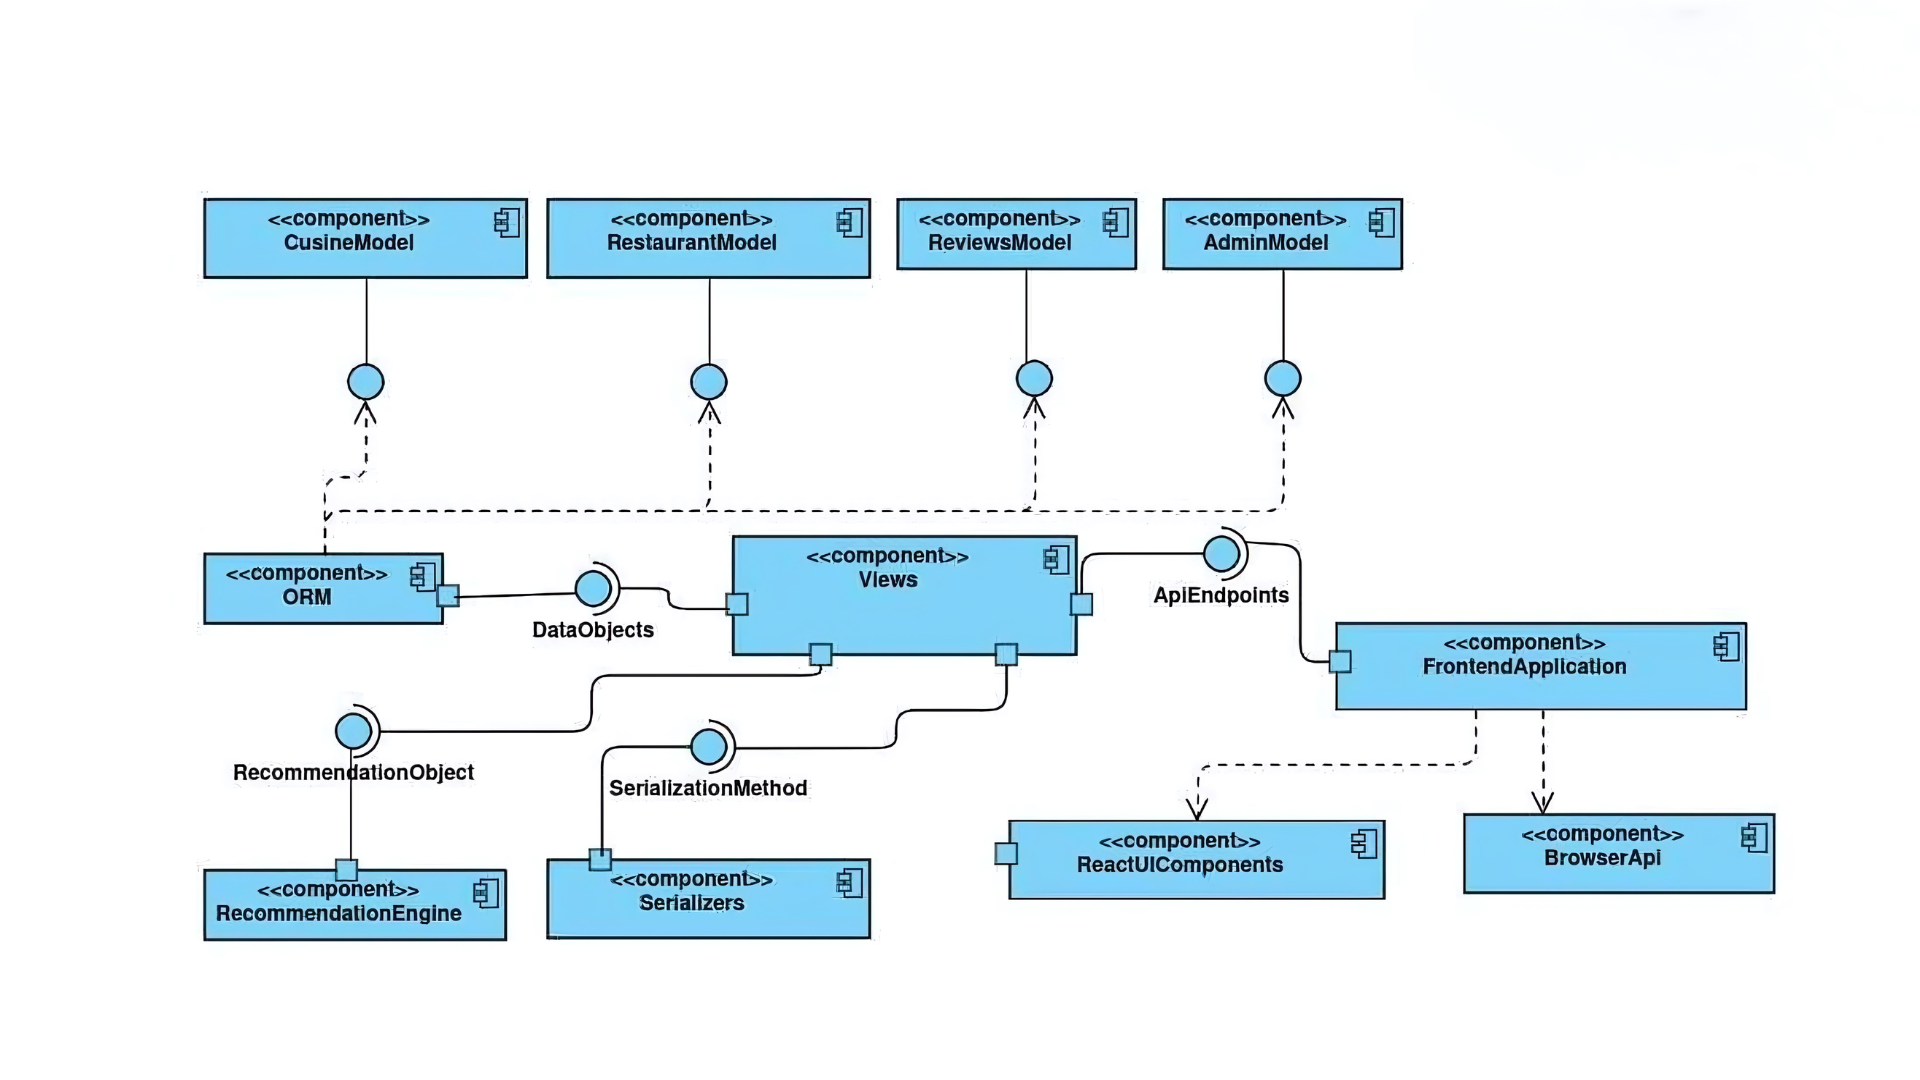
\includegraphics[width=0.9\textheight]{component}}
    \caption{Component Diagram}
    \label{fig:component}
\end{figure}

\pagebreak

% \subsection{Deployment Diagram Explanation}

% This deployment diagram represents the architecture of the FoodFind project. It shows the physical deployment of the software components on different nodes. Here's a brief explanation of the components and their interactions:

% \subsubsection*{Components}
% \begin{itemize}
%     \item \textbf{Server Node}
%     \begin{itemize}
%         \item The entire deployment is encapsulated within a server node.
%     \end{itemize}

%     \item \textbf{nginx}
%     \begin{itemize}
%         \item \textbf{Type}: Execution Environment
%         \item \textbf{Component}: \texttt{web-ui}
%         \item This component represents the web server that serves the front-end part of the application.
%         \item It handles HTTP requests and forwards API requests to the Django backend.
%         \item The front-end UI interacts with the users and sends requests to the Django backend through the API.
%     \end{itemize}

%     \item \textbf{Django}
%     \begin{itemize}
%         \item \textbf{Type}: Interface (\texttt{Server::API})
%         \item \textbf{Component}: \texttt{Django}
%         \item This component represents the backend of the application implemented using the Django framework.
%         \item It handles the business logic and processes API requests received from the \texttt{web-ui}.
%         \item Communicates with the PostgreSQL database to fetch and store data.
%     \end{itemize}

%     \item \textbf{PostgreSQL}
%     \begin{itemize}
%         \item \textbf{Type}: Execution Environment
%         \item \textbf{Component}: \texttt{PostgreSql}
%         \item This component represents the database server where all the application's data is stored.
%         \item The Django backend interacts with this database to perform CRUD (Create, Read, Update, Delete) operations.
%     \end{itemize}
% \end{itemize}

% \subsubsection*{Interactions}
% \begin{itemize}
%     \item The \textbf{nginx} server hosts the \texttt{web-ui} component and forwards API requests to the Django backend.
%     \item The \textbf{Django} component acts as an API server, processing incoming requests and interacting with the PostgreSQL database.
%     \item The \textbf{PostgreSQL} database stores all the data related to the application, such as user information, restaurant details, reviews, etc.
% \end{itemize}


% \begin{figure}[H]
%     \centering
%     \includegraphics[width=\textwidth]{deployment.png}
%     \caption{Deployment Diagram}
%     \label{fig:deploymentdiag}
% \end{figure}
% This deployment diagram provides a clear overview of how the FoodFind project is structured and deployed. The front-end UI is served by the nginx server, which interacts with the Django backend to process requests. The Django backend, in turn, communicates with the PostgreSQL database to manage the application's data. This setup ensures a clear separation of concerns and a scalable architecture for handling user interactions and data management efficiently.
% \pagebreak






\section{Technologies Used}
 Table \ref{table:tech} consists of the major technologies that are being used for development and deployment of the application. They are briefly described in the subsections that follow.

 \renewcommand{\arraystretch}{1.5}
 \begin{table}[H]
 \begin{tabular}{|l|l|}
 \hline
 \rowcolor[HTML]{C0C0C0} 
 \textbf{Subject}    & \textbf{Tools and Technologies Used} \\ \hline
 Backend Database            & SQLite                        \\ \hline
 REST API Service    & Django REST Framework; Postman        \\ \hline
 Web Application  & Vite; TypeScript                 \\ \hline
 IDE / Code Editor& Sublime Text; Code-OSS  \\ \hline
 Version Control System& GitHub  \\ \hline
 Documentation & Overleaf \\ \hline
 \end{tabular}
 \caption{Technologies Being Used}
 \label{table:tech}
 \end{table}

 \subsection{SQLite}
   SQLite provides a reliable and efficient database solution for storing user profiles, restaurant details, and reviews. Its serverless architecture is ideal for the FoodFind app, which requires a lightweight database that can handle high traffic and complex queries with ease.

  \subsection{Django REST Framework}
    The Django REST Framework will serve as the backbone for the FoodFind API, handling data serialization and request processing. It will enable seamless communication between the app's frontend and the SQLite database, ensuring a smooth user experience.

  \subsection{Postman}
    Postman will be utilized during development to test and refine the FoodFind API. It will help ensure that the API endpoints return the correct data and handle errors properly, which is crucial for the reliability of the app.

  \subsection{Vite}
    Vite will accelerate the development process of FoodFind by providing a fast and modern build system. Its hot module replacement feature will allow developers to see changes in real-time, enhancing productivity.

  \subsection{TypeScript}
    TypeScript will be used to write scalable and maintainable code for the FoodFind web app. Its static typing system will help catch errors early in development, leading to a more robust and error-free application.

  \subsection{Sublime Text}
    Sublime Text will be the code editor of choice for developers working on FoodFind due to its speed and efficiency. Its vast array of plugins will aid in writing clean and optimized code for the project.

  \subsection{Code-OSS}
    Code-OSS will provide a comprehensive development environment for the FoodFind project. Its support for debugging, version control, and extensions will contribute to an efficient development workflow.

   \subsection{GitHub}
     GitHub will be essential for version control and collaboration among the FoodFind development team. It will track changes, manage code contributions, and host the project's repository, facilitating teamwork and progress tracking.

   \subsection{Overleaf}
     Overleaf will be used to create and maintain the FoodFind project's documentation. Its real-time collaboration features will allow multiple contributors to work on the documentation simultaneously, ensuring it stays up-to-date and comprehensive.
\pagebreak


\section{Recommendation Algorithms}
The recommendation system in the FoodFind project is designed to provide personalized restaurant suggestions to users based on their preferences and interactions. The algorithm employs a hybrid approach, combining collaborative filtering and content-based filtering techniques
\subsection{Data Retrieval}

The algorithm starts by retrieving relevant data based on user interactions and specified parameters:
\begin{itemize}
    \item \textbf{User ID}: Identifies the user for whom recommendations are to be generated.
    \item \textbf{Recommendation Flag}: Determines if recommendations are requested.
    \item \textbf{Tags}: Filters restaurants based on specified tags.
\end{itemize}

\subsection{Collaborative Filtering}

Collaborative filtering generates recommendations by identifying similarities between users. This involves:
\begin{itemize}
    \item \textbf{User Favorites and Reviews}: Collecting the list of favorite restaurants and reviews for the specified user.
    \item \textbf{Identifying Similar Users}: Finding other users who share similar tastes by checking for overlapping favorite restaurants and reviewed restaurants.
    \item \textbf{Generating Collaborative Recommendations}: Recommending restaurants that are liked or reviewed by these similar users but not by the current user.
\end{itemize}

\subsection{Content-Based Filtering}

Content-based filtering uses the attributes of restaurants to find items similar to those the user already likes:
\begin{itemize}
    \item \textbf{User Tags}: Identifying tags associated with the user’s favorite restaurants.
    \item \textbf{Generating Content Recommendations}: Selecting restaurants that match these tags, ensuring they share characteristics with those that the user has already shown interest in.
\end{itemize}

\subsection{Combining Recommendations: Hybrid Filtering}

The algorithm combines the results from collaborative filtering and content-based filtering:
\begin{itemize}
    \item \textbf{Union of Recommendations}: Merging the collaborative and content-based recommendations to form a unique set of suggested restaurants.
\end{itemize}

\subsection{Annotation and Sorting}

To present the most relevant recommendations, the algorithm:
\begin{itemize}
    \item \textbf{Annotates Recommendations}: Adds metadata such as average ratings and the number of reviews to each restaurant.
    \item \textbf{Sorting}: Orders the restaurants by average rating and review count, ensuring the highest-rated and most-reviewed options are prioritized.
\end{itemize}

\subsection{Handling No Recommendations}

If the algorithm does not generate any specific recommendations, it defaults to returning the entire list of available restaurants, ensuring that the user always receives some suggestions.

\pagebreak
\section{Performance Analysis Methodology}

In order to make this project effective and robust, we will be making sure it adheres to top notch quality by testing it with different performance metrics, validation scheme and benchmark tests. 

\subsection{Data Management}
A detailed database of restaurants and cafes will be manually compiled, including information such as menus, special deals, and events. This database will not only facilitate efficient data access but also enable comprehensive analysis of dining trends and customer preferences.

\subsection{API Development}
A robust API service will be developed using the Django REST Framework, with testing conducted through Postman to ensure seamless data retrieval and display. This API will dynamically generate profiles for each restaurant, pulling real-time data from the backend to provide up-to-date information without the need for manual profile creation.

\subsection{Web Application Functionality}
The front-end will be crafted using Vite and TypeScript, focusing on a responsive and interactive user experience. Emphasis will be placed on creating an intuitive design that adapts to different devices, ensuring accessibility and ease of use for all users.
\pagebreak


\section{Risk Analysis}

Risk analysis for the FoodFind project involves identifying potential risks, assessing their impact, and devising strategies to mitigate them. This section covers both technical and operational risks.

\subsection{Technical Risks}

\begin{table}[H]
\centering
\caption{Technical Risks}
\begin{tabularx}{\textwidth}{|p{0.25\textwidth}|X|X|}
\hline
\textbf{Risk} & \textbf{Description} & \textbf{Mitigation} \\
\hline
Security Vulnerabilities & Unsecured API endpoints may expose the application to data breaches, unauthorized access, and data manipulation. & Implement secure API practices such as HTTPS, token-based authentication, and regular security audits. \\
\hline
Scalability Issues & The initial architecture may not handle increased user load as the app gains popularity. & Design the system with scalability in mind, use load balancers, and implement efficient database indexing and caching strategies. \\
\hline
Data Accuracy and Consistency & Inaccurate or inconsistent data about restaurants could lead to user dissatisfaction. & Implement rigorous data validation processes and regular data audits to ensure accuracy and consistency. \\
\hline
Performance Bottlenecks & High traffic or complex queries could lead to slow response times. & Optimize the code, use performance monitoring tools, and conduct regular load testing to identify and resolve bottlenecks. \\
\hline
Technical Debt & Accumulation of quick fixes and suboptimal code may hamper future development and maintenance. & Follow best coding practices, conduct regular code reviews, and allocate time for refactoring. \\
\hline
\end{tabularx}
\label{tab:technical-risks}
\end{table}

\subsection{Operational Risks}

\begin{table}[H]
\centering
\caption{Operational Risks}
\begin{tabularx}{\textwidth}{|p{0.25\textwidth}|X|X|}
\hline
\textbf{Risk} & \textbf{Description} & \textbf{Mitigation} \\
\hline
User Engagement and Participation & Low user engagement may affect the quality and quantity of reviews and recommendations. & Implement user engagement strategies such as rewards for active participation, regular updates, and interactive features. \\
\hline
Resource Constraints & Limited resources (time, budget, personnel) may affect the development and operational aspects. & Prioritize tasks, allocate resources efficiently, and seek additional funding or partnerships if necessary. \\
\hline
Regulatory Compliance & Non-compliance with local laws and regulations could result in legal issues. & Stay informed about relevant laws and regulations, and ensure the app complies with all legal requirements. \\
\hline
Technological Changes & Rapid changes in technology may render some components of the app obsolete. & Stay updated with technological trends, be prepared to adapt, and invest in continuous learning and development. \\
\hline
\end{tabularx}
\label{tab:operational-risks}
\end{table}
\pagebreak




% \subsection{Outputs}
% The Landing Page serves as the entry point for users, offering an interface that allows users to log in to the application. For user login Google Oauth Api is used to get user details from google server.
% \vspace{2mm}
% \begin{figure}[h]
% 	\includegraphics[width=\linewidth]{landingpage}
% 	\centering
% 	\caption{Home Page}
% 	\label{fig:Home Page}
% \end{figure}
% \pagebreak

% The Page to View Restaurants lists all available restaurants, providing users with a comprehensive overview of their options. This page includes essential information such as restaurant names, images, and brief descriptions. Users can easily filter and sort the list based on tags. The page communicates with API endpoint setup for fetching all the restaurant details.
% \vspace{2mm}
% \begin{figure}[h]
% 	\includegraphics[width=0.9\textwidth]{restaurants}
% 	\centering
% 	\caption{Restaurants List}
% 	\label{fig:Restaurant}
% \end{figure}
% \pagebreak

% The Page to View Restaurant Details offers in-depth information about each restaurant. When a user selects a restaurant from the list, they are directed to this page, which includes detailed descriptions, full menus, customer reviews, operating hours, and more. High-quality images of the restaurant are displayed to provide users with a sense of what to expect. This page also integrates interactive elements, such as a map showing the restaurant’s location. It also hits an API endpoint for the restaurant details data.
% \vspace{2mm}
% \begin{figure}[h]
% 	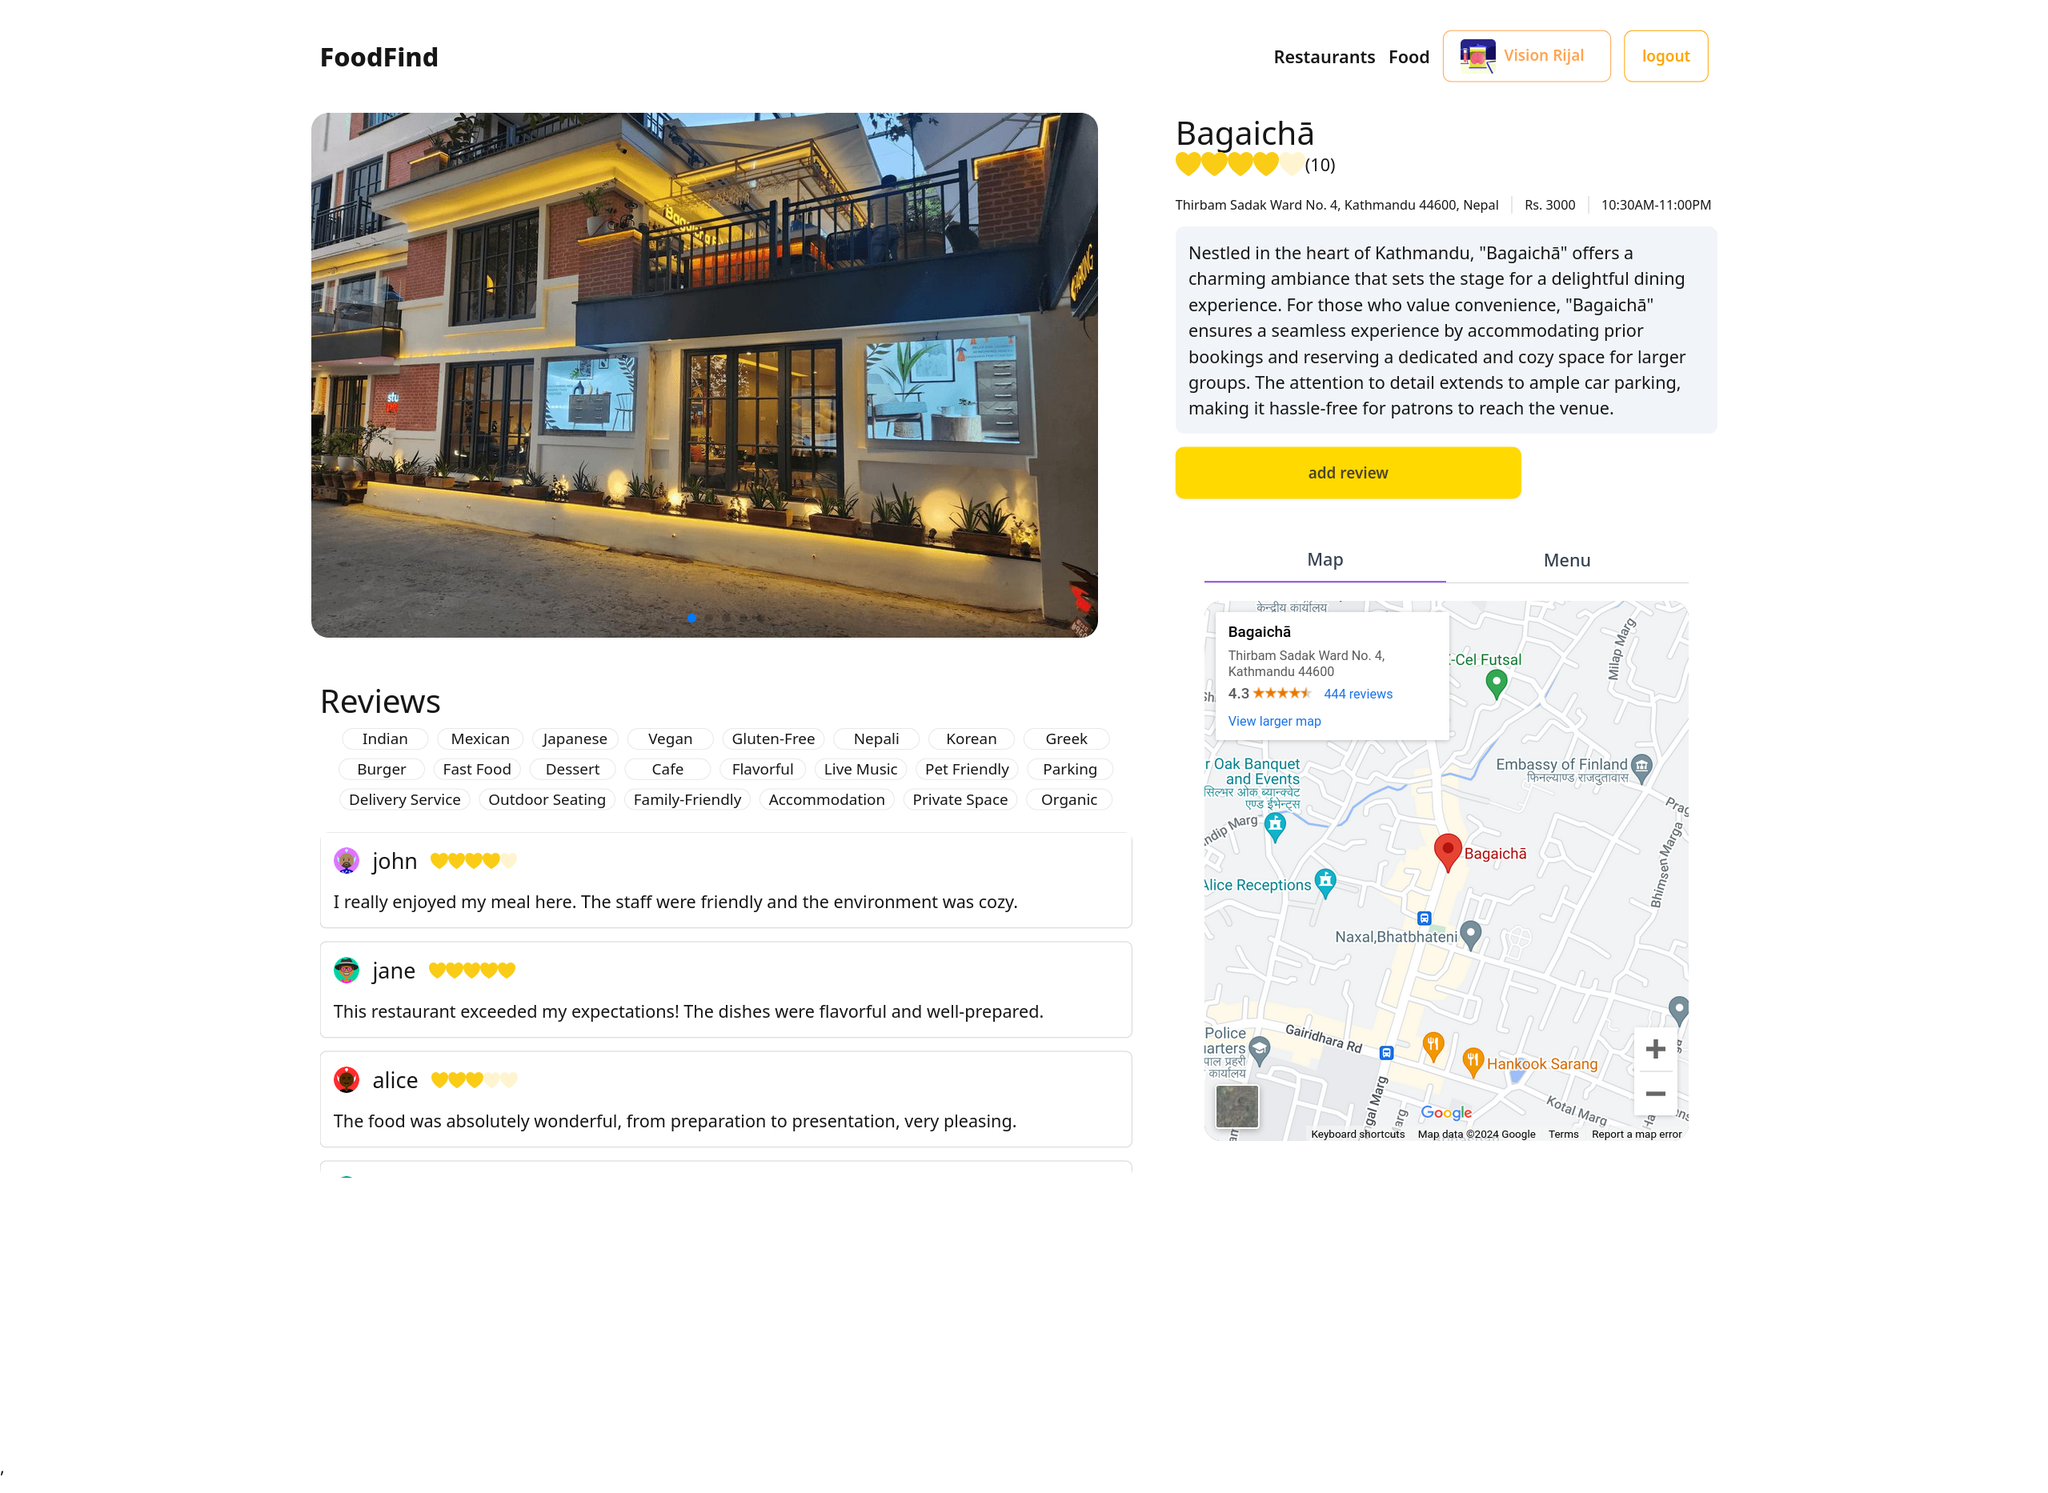
\includegraphics[width=\linewidth]{reviewsdiag}
% 	\centering
% 	\caption{Providing Review}
% 	\label{fig:Review}
% \end{figure}
% \pagebreak


\section{Test Cases}
This section outlines the test cases for the FoodFind web application. The scope of testing includes functionality related to searching, reviewing, and marking restaurants as favorites.

\subsection{Features to be Tested}
\begin{itemize}
	\item Restaurant profiles
	\item Review and rating
	\item Add and remove favorite restaurants
	\item Map section for searching and suggesting nearby restaurants
	\item Restaurant addition by users
	\item Filtering restaurants based on tags
	\item Admin panel functionalities
	\item User profile section
	\item Google authentication login
\end{itemize}

\subsection{Test Case Format Description}
Each test case is described with the following details:
\begin{itemize}
	\item \textbf{Test Case ID} - Unique identifier for the test case.
	\item \textbf{Description} - Overview of what is being tested.
	\item \textbf{Test Steps} - Steps to execute the test.
	\item \textbf{Expected Result} - Expected outcome of the test.
	\item \textbf{Actual Result} - Actual outcome of the test.
\end{itemize}

\subsection{Test Cases}

\subsubsection{Restaurant Profiles}
\captionsetup{type=table}
\begin{tabularx}{\textwidth}{|X|X|X|X|X|}
	\hline
	\rowcolor{gray}
	\textbf{Test Case ID} & \textbf{Description} & \textbf{Test Steps} & \textbf{Expected Result} & \textbf{Actual Result} \\ \hline
	TC1 & View restaurant details & 
    \begin{itemize}[left=0pt, nosep]
        \item Navigate to the search page.
        \item Enter the restaurant name and search.
        \item Click on a restaurant to view details.
    \end{itemize}
    & Restaurant details are displayed correctly. & Restaurant details displayed as expected, including name, address, and contact information. \\ \hline
	TC2 & View restaurant menu & 
    \begin{itemize}[left=0pt, nosep]
        \item Click on the 'Menu' tab.
    \end{itemize}
    & The menu for the restaurant is displayed with prices and items. & Menu displayed correctly with all items and prices listed. \\ \hline
\end{tabularx}
\captionof{table}{Test Cases for Restaurant Profiles}
\label{tab:restaurant-profiles}

\subsubsection{Review and Rating}
\captionsetup{type=table}
\begin{tabularx}{\textwidth}{|X|X|X|X|X|}
	\hline
	\rowcolor{gray}
	\textbf{Test Case ID} & \textbf{Description} & \textbf{Test Steps} & \textbf{Expected Result} & \textbf{Actual Result}  \\ \hline
	TC3 & Add a review to a restaurant & 
    \begin{itemize}[left=0pt, nosep]
        \item Click on the 'Write Review' button.
        \item Enter review text and rating.
        \item Submit the review.
    \end{itemize}
    & Review is saved and displayed under the restaurant profile. & Review was successfully submitted and is visible on the restaurant’s profile with correct text and rating. \\ \hline
	TC4 & View reviews for a restaurant & 
    \begin{itemize}[left=0pt, nosep]
        \item Scroll to the reviews section.
    \end{itemize}
    & User reviews are displayed with ratings. & Reviews are displayed with correct user names, text, and ratings. \\ \hline
\end{tabularx}
\captionof{table}{Test Cases for Review and Rating}
\label{tab:review-rating}

\subsubsection{Add and Remove Favorite Restaurant}
\captionsetup{type=table}
\begin{tabularx}{\textwidth}{|X|X|X|X|X|}
	\hline
	\rowcolor{gray}
	\textbf{Test Case ID} & \textbf{Description} & \textbf{Test Steps} & \textbf{Expected Result} & \textbf{Actual Result} \\ \hline
	TC5 & Add restaurant to favorites & 
    \begin{itemize}[left=0pt, nosep]
        \item Click on the 'Add to Favorites' button.
    \end{itemize}
    & Restaurant is added to the user's favorite list. & Restaurant was successfully added to the favorite list and appears under the 'Favorites' section. \\ \hline
	TC6 & Remove restaurant from favorites & 
    \begin{itemize}[left=0pt, nosep]
        \item Click on the 'Remove from Favorites' button.
    \end{itemize}
    & Restaurant is removed from the user's favorite list. & Restaurant was successfully removed from the favorite list and no longer appears under 'Favorites'. \\ \hline
\end{tabularx}
\captionof{table}{Test Cases for Adding and Removing Favorite Restaurants}
\label{tab:fav-restaurant}

\subsubsection{Map Section}
\captionsetup{type=table}
\begin{tabularx}{\textwidth}{|X|X|X|X|X|}
	\hline
	\rowcolor{gray}
	\textbf{Test Case ID} & \textbf{Description} & \textbf{Test Steps} & \textbf{Expected Result} & \textbf{Actual Result} \\ \hline
	TC7 & Automatically display nearby restaurants on the map & 
    \begin{itemize}[left=0pt, nosep]
        \item Open the map page.
    \end{itemize}
    & The map automatically shows restaurants within a 3 km radius along with routes and distances from the user's current location. & Nearby restaurants were displayed correctly on the map with accurate routes and distances. \\ \hline
	TC8 & Search for a specific restaurant on the map & 
    \begin{itemize}[left=0pt, nosep]
        \item Enter the restaurant name in the search bar.
        \item Select the desired restaurant from suggestions.
    \end{itemize}
    & The route and distance to the selected restaurant from the user's current location are displayed on the map. & Route and distance to the selected restaurant were displayed accurately on the map. \\ \hline
\end{tabularx}
\captionof{table}{Test Cases for Map Section}
\label{tab:map-section}

\subsubsection{Restaurant Addition by Users}
\captionsetup{type=table}
\begin{tabularx}{\textwidth}{|X|X|X|X|X|}
	\hline
	\rowcolor{gray}
	\textbf{Test Case ID} & \textbf{Description} & \textbf{Test Steps} & \textbf{Expected Result} & \textbf{Actual Result} \\ \hline
	TC9 & Add a new restaurant & 
    \begin{itemize}[left=0pt, nosep]
        \item Click on the 'Add Restaurant' button.
        \item Fill in the restaurant details (name, location, menu, etc.).
        \item Submit the form.
    \end{itemize}
    & Restaurant data is submitted to the admin for review. & Restaurant was successfully added and appears in search results with correct details. \\ \hline
\end{tabularx}
\captionof{table}{Test Cases for Restaurant Addition by Users}
\label{tab:restaurant-addition}

\subsubsection{Filtering Restaurants Based on Tags}
\captionsetup{type=table}
\begin{tabularx}{\textwidth}{|X|X|X|X|X|}
	\hline
	\rowcolor{gray}
	\textbf{Test Case ID} & \textbf{Description} & \textbf{Test Steps} & \textbf{Expected Result} & \textbf{Actual Result} \\ \hline
	TC10 & Filter restaurants by tag & 
    \begin{itemize}[left=0pt, nosep]
        \item Go to the filter section.
        \item Select a tag from the available options.
        \item Apply the filter.
    \end{itemize}
    & Restaurants matching the selected tag are displayed. & Restaurants filtered correctly based on the selected tag and displayed as expected. \\ \hline
\end{tabularx}
\captionof{table}{Test Cases for Filtering Restaurants Based on Tags}
\label{tab:filter-tags}

\subsubsection{Admin Panel Functionalities}
\captionsetup{type=table}
\begin{tabularx}{\textwidth}{|X|X|X|X|X|}
	\hline
	\rowcolor{gray}
	\textbf{Test Case ID} & \textbf{Description} & \textbf{Test Steps} & \textbf{Expected Result} & \textbf{Actual Result} \\ \hline
	TC11 & Admin access to restaurant and user management & 
    \begin{itemize}[left=0pt, nosep]
        \item Log in as an admin.
        \item Navigate to the restaurant or user management section.
        \item View, edit, or delete restaurant or user entries.
    \end{itemize}
    & Admin can view, edit, and delete restaurant or user details. & Admin access works as intended; restaurant and user entries can be managed correctly. \\ \hline
\end{tabularx}
\captionof{table}{Test Cases for Admin Panel Functionalities}
\label{tab:admin-panel}

\subsubsection{User Profile Section}
\captionsetup{type=table}
\begin{tabularx}{\textwidth}{|X|X|X|X|X|}
	\hline
	\rowcolor{gray}
	\textbf{Test Case ID} & \textbf{Description} & \textbf{Test Steps} & \textbf{Expected Result} & \textbf{Actual Result} \\ \hline
	TC12 & View and edit user profile & 
    \begin{itemize}[left=0pt, nosep]
        \item Log in as a user.
        \item Go to the user profile section.
        \item View the user info, reviews provided and the favorite restaurants.
    \end{itemize}
    & User profile details are displayed. & User profile section displayed. \\ \hline
\end{tabularx}
\captionof{table}{Test Cases for User Profile Section}
\label{tab:user-profile}

\subsubsection{Google Authentication Login}
\captionsetup{type=table}
\begin{tabularx}{\textwidth}{|X|X|X|X|X|}
	\hline
	\rowcolor{gray}
	\textbf{Test Case ID} & \textbf{Description} & \textbf{Test Steps} & \textbf{Expected Result} & \textbf{Actual Result} \\ \hline
	TC13 & Google authentication login & 
    \begin{itemize}[left=0pt, nosep]
        \item Go to the login page.
        \item Click on 'Login with Google'.
        \item Authenticate with Google credentials.
    \end{itemize}
    & User is logged in and redirected to the homepage. & Google authentication worked; user logged in successfully and redirected to the homepage. \\ \hline
\end{tabularx}
\captionof{table}{Test Cases for Google Authentication Login}
\label{tab:google-authentication}

\pagebreak


\section{Project Task and Time Schedule}
The working time period for the project was four months, spanning the entire duration of the spring semester. The project was structured to ensure all tasks were completed in a timely manner, adhering to the university's requirements. The project timeline was divided into various phases, including planning, development, testing, and deployment. Each phase had specific milestones that the team aimed to achieve within set deadlines. This structured approach ensured efficient progress and timely completion of the project..
\subsection{Division of Roles and Responsibilities}
The success of the project heavily relied on the effective collaboration of all team members, each assigned specific roles and responsibilities. The roles were divided based on the expertise and skills of each member to ensure optimal contribution to the project. Table \ref{table:team-roles} outlines the division of roles and responsibilities among the team members.
\begin{table}[!ht]
\begin{tabularx}{\textwidth}{|c|l|l|X|}
    \hline
    \rowcolor[HTML]{C0C0C0} 
    \textbf{S.N.} & \textbf{Team Member} & \textbf{Role} & \textbf{Responsibilities} \\ \hline
    1. & Pradip Dhungana & Backend Developer & 
    \begin{itemize}
        \item Admin Panel and develop API endpoints to handle requests from and send responses to the web application.
        \item Manage the database and handle documentation.
    \end{itemize}
    \\ \hline
    2. & Vision Rijal & Frontend Developer & 
    \begin{itemize}
        \item Prepare the User Interface (UI) of the web application.
        \item Manage the project team and guide the team along various phases of project development.
    \end{itemize}
    \\ \hline
    3. & Bishnu Timilsena & Backend Developer &  
    \begin{itemize}
        \item Develop API endpoints for dynamic pages. Test and ensure validity and security of API endpoints.
        \item Handle data collection tasks.
    \end{itemize}
    \\ \hline
\end{tabularx}
\caption{Division of Roles and Responsibilities of Team Members}
\label{table:team-roles}
\end{table}
\pagebreak
\subsection{Gantt Chart}
The time schedule for the development of the project is illustrated in the
following figures.
 \begin{figure}[h!]
	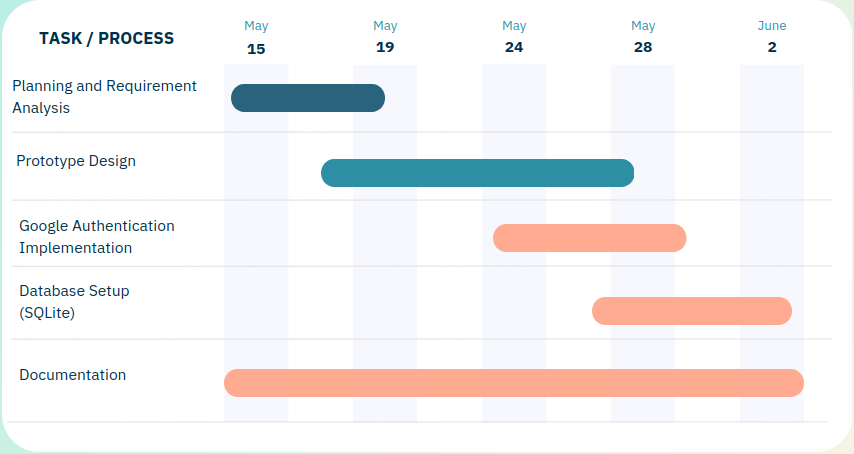
\includegraphics[width=\linewidth]{images/1.png}
	\centering
	\caption{Gantt Chart for increment 1}
	\label{fig:schedule1}
 \end{figure}
 \begin{figure}[h!]
	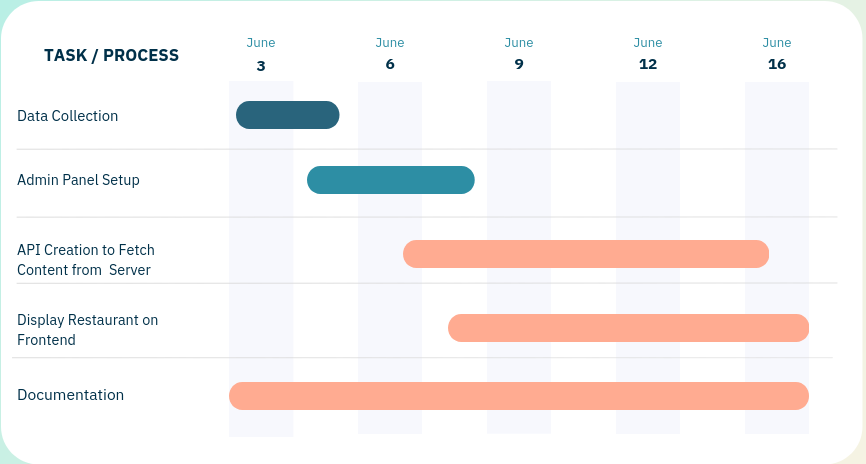
\includegraphics[width=\linewidth]{images/2.png}
	\centering
	\caption{Gantt Chart for increment 2}
	\label{fig:schedule2}
 \end{figure}
 \begin{figure}[h!]
	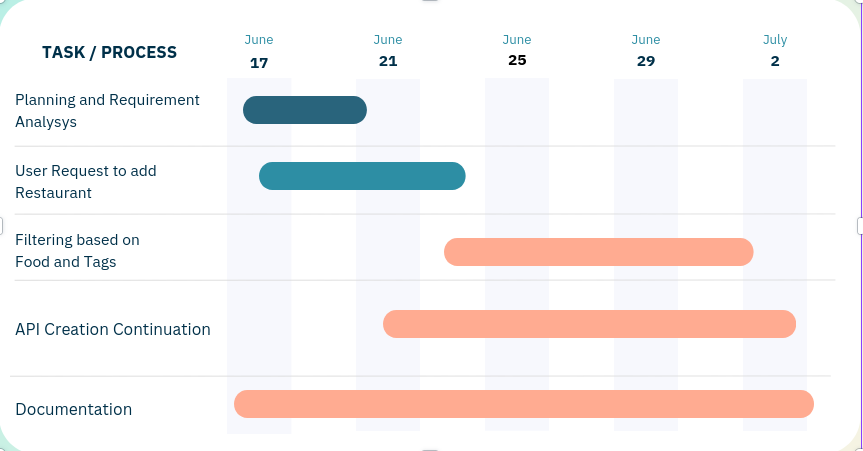
\includegraphics[width=\linewidth]{images/3.png}
	\centering
	\caption{Gantt Chart for increment 3}
	\label{fig:schedule3}
 \end{figure}
 \begin{figure}[h!]
	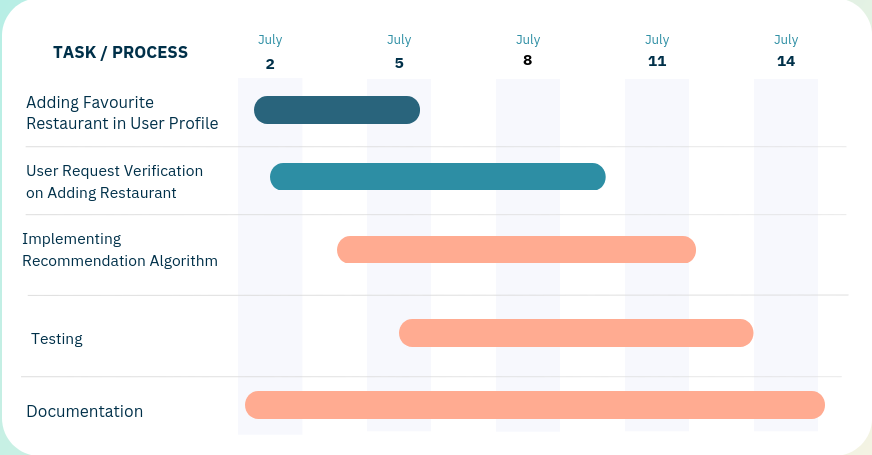
\includegraphics[width=\linewidth]{images/4.png}
	\centering
	\caption{Gantt Chart for increment 4}
	\label{fig:schedule4}
 \end{figure}
\clearpage
\pagebreak
\section{Deliverable/Output}

As per our objective, we have developed a web-based platform, FoodFind, which helps restaurant owners to showcase their dining establishments and provides a platform for customers to discover and choose the best dining options. This platform allows restaurant owners to publish detailed information about their eateries, while offering customers the convenience of selecting their desired dining venue from the comfort of their homes, thus saving time and effort.

\subsection{Search and Discovery}
The primary feature of FoodFind is its robust search functionality. Users can effortlessly locate restaurants by entering a name or selecting a location. This search process is designed to be intuitive and accessible to all users, regardless of their technical expertise.

\subsection{Filtering Options}
The platform includes advanced filtering options, allowing users to refine their searches based on specific criteria such as cuisine type and location. This functionality makes it easier for users to find restaurants that meet their specific tastes and preferences.

\subsection{Menu and Pricing Information}
FoodFind offers comprehensive information on restaurant menus and pricing. This transparency allows users to make well-informed dining decisions based on their budget and food preferences, enhancing their overall dining experience.

\subsection{User Reviews and Sharing}
While FoodFind does not host internal community postings, it enables users to share their dining experiences on external platforms. This feature encourages community-driven recommendations and helps users make better dining choices.
\subsection{AI-Powered Recommendations} I
Provides personalized restaurant suggestions based on user preferences and past behavior, leveraging advanced machine learning algorithms to enhance recommendation accuracy and user satisfaction.
\subsection{Personalized Favorite Restaurant Bookmarking}
FoodFind offers a feature that allows users to add their favorite restaurants to their profiles for easy access. This functionality enables users to bookmark and revisit their preferred dining establishments without the need to search for them again, enhancing user convenience and engagement.

\subsection{User-Friendly Interface}
FoodFind boasts a user-friendly interface designed to provide a seamless browsing experience. The platform is optimized for both desktop and mobile use, ensuring accessibility across different devices.

\subsection{Support for Local Establishments}
FoodFind plays a crucial role in promoting local restaurants. By featuring these establishments, the platform helps increase their visibility, driving growth and fostering customer engagement, which is beneficial for the local economy.

\subsection{Integration with Maps}
FoodFind integrates with mapping services, allowing users to view restaurant locations and get directions easily. This feature adds a layer of convenience for users planning their dining experiences.
\pagebreak


\section{Conclusion}

The FoodFind project has successfully met its objectives of developing a comprehensive web-based platform that enhances the dining experience in Kathmandu. By leveraging advanced search functionalities, detailed menu and pricing information, user reviews, and a user-friendly interface, FoodFind provides a robust solution for discovering and choosing dining options that best suit users' preferences.

The platform effectively supports local restaurants by increasing their visibility and customer engagement. Features such as search and discovery, filtering options, and integration with mapping services contribute to a seamless user experience, allowing users to make informed dining decisions effortlessly.

The successful completion of the FoodFind project demonstrates its potential to transform the dining landscape in Kathmandu. The platform is poised to become a valuable resource for both users seeking quality dining experiences and local establishments looking to reach a broader audience. We are confident that FoodFind will significantly contribute to a more connected and enjoyable dining community.
\pagebreak

\section{Future Enhancements}

To ensure continuous improvement and adaptability, the following future enhancements are planned for FoodFind:

\begin{itemize}
  
    \item \textbf{Reservation System:} Introducing an integrated reservation system that allows users to book tables directly through the platform.
    \item \textbf{Expanded Reviews:} Hosting community reviews to provide more comprehensive insights into dining experiences.
    \item \textbf{Real-Time Updates:} Offering real-time updates on restaurant availability and promotions to keep users informed about the latest dining options and special deals.
\end{itemize}

These enhancements will further solidify FoodFind's position as a leading platform for restaurant discovery and dining experiences, continually evolving to meet the needs of its users and the local restaurant community.
\pagebreak

\addcontentsline{toc}{section}{REFERENCES}
\bibliography{references}
\bibliographystyle{ieeetran}
\pagebreak
\addcontentsline{toc}{section}{APPENDIX A}
\appendix
\section*{APPENDIX A}

\subsection*{Endpoint: /restaurants/}
\textbf{Method:} GET \\
\textbf{Description:} Retrieve a list of restaurants. If \texttt{recommend=true} is provided, it retrieves recommended restaurants for the specified \texttt{user\_id}. If \texttt{tags} are provided, it filters restaurants based on tags. \\
\textbf{Request Parameters:} \texttt{recommend=true} and \texttt{user\_id=\{user\_id\}} OR \texttt{tags=[tag1, tag2]} \\
\textbf{Request Body:} - \\
\textbf{Response:} \\
\texttt{[ \{"id": 1, "name": "Restaurant Name", "location": "Location", "description": "Description", "images": [\{"id": 1, "image": "image\_url"\}]\} ]} \\
OR \\
\texttt{ \{"images": [\{"id": 1, "image": "image\_url"\}], "id": 1, "name": "Restaurant Name", "location": "Location", "price": "Price", "opening\_hours": "Opening Hours", "description": "Description", "average\_rating": 4.5, "reviews": [\{"id": 1, "user": \{"id": 1, "username": "User Name", "email": "user@example.com", "profile\_picture": "profile\_picture\_url"\}, "rating": 5, "review\_text": "Review text", "created\_at": "2024-07-25T05:33:38.644Z", "updated\_at": "2024-07-25T05:33:38.644Z", "restaurant\_name": "Restaurant Name", "restaurant\_id": 1}\], "map\_url": "Map URL", "menu\_items": [\{"id": 1, "name": "Menu Item", "price": "Price", "category": "Category"\}], "no\_of\_reviews": 10, "tags": [\{"id": 1, "name": "Tag"\}]\} }

\subsection*{Endpoint: /restaurants/\{id\}/}
\textbf{Method:} GET \\
\textbf{Description:} Retrieve details of a specific restaurant. \\
\textbf{Request Parameters:} - \\
\textbf{Request Body:} - \\
\textbf{Response:} \\
\texttt{ \{"images": [\{"id": 1, "image": "image\_url"\}], "id": 1, "name": "Restaurant Name", "location": "Location", "price": "Price", "opening\_hours": "Opening Hours", "description": "Description", "average\_rating": 4.5, "reviews": [\{"id": 1, "user": \{"id": 1, "username": "User Name", "email": "user@example.com", "profile\_picture": "profile\_picture\_url"\}, "rating": 5, "review\_text": "Review text", "created\_at": "2024-07-25T05:33:38.644Z", "updated\_at": "2024-07-25T05:33:38.644Z", "restaurant\_name": "Restaurant Name", "restaurant\_id": 1}\], "map\_url": "Map URL", "menu\_items": [\{"id": 1, "name": "Menu Item", "price": "Price", "category": "Category"\}], "no\_of\_reviews": 10, "tags": [\{"id": 1, "name": "Tag"\}]\} }

\subsection*{Endpoint: /toprestaurants/}
\textbf{Method:} GET \\
\textbf{Description:} Retrieve a list of top restaurants. \\
\textbf{Request Parameters:} - \\
\textbf{Request Body:} - \\
\textbf{Response:} \\
\texttt{[ \{"id": 1, "restaurant": \{"id": 1, "name": "Restaurant Name", "location": "Location", "description": "Description", "images": [\{"id": 1, "image": "image\_url"\}]\}, "ranking": 1\} ]}

\subsection*{Endpoint: /tags/}
\textbf{Method:} GET \\
\textbf{Description:} Retrieve a list of all tags. \\
\textbf{Request Parameters:} - \\
\textbf{Request Body:} - \\
\textbf{Response:} \\
\texttt{[ \{"id": 1, "name": "Tag Name"\} ]}

\subsection*{Endpoint: /google-login/}
\textbf{Method:} POST \\
\textbf{Description:} Authenticate user via Google login. \\
\textbf{Request Parameters:} - \\
\textbf{Request Body:} \\
\texttt{\{"token": "Google OAuth Token"\}} \\
\textbf{Response:} \\
\texttt{\{"id": 1, "username": "User Name", "email": "user@example.com", "profile\_picture": "profile\_picture\_url", "favorite\_restaurants": [7, 8, 9]\}}

\subsection*{Endpoint: /create-review/}
\textbf{Method:} POST \\
\textbf{Description:} Create or update a review for a restaurant. \\
\textbf{Request Parameters:} - \\
\textbf{Request Body:} \\
\texttt{\{"user": 1, "rating": 5, "review\_text": "Great place!", "restaurant": 1\}} \\
\textbf{Response:} \\
\texttt{\{"id": 1, "user": 1, "rating": 5, "review\_text": "Great place!", "created\_at": "2024-07-25T05:33:38.644Z", "updated\_at": "2024-07-25T05:33:38.644Z", "restaurant\_id": 1\}}

\subsection*{Endpoint: /user-reviews/\{user_id\}/}
\textbf{Method:} GET \\
\textbf{Description:} Retrieve all reviews created by a specific user. \\
\textbf{Request Parameters:} - \\
\textbf{Request Body:} - \\
\textbf{Response:} \\
\texttt{[ \{"id": 1, "user": \{"id": 1, "username": "User Name", "email": "user@example.com", "profile\_picture": "profile\_picture\_url"\}, "rating": 5, "review\_text": "Great place!", "created\_at": "2024-07-25T05:33:38.644Z", "updated\_at": "2024-07-25T05:33:38.644Z", "restaurant\_name": "Restaurant Name", "restaurant\_id": 1\} ]}

\subsection*{Endpoint: /add-to-favorites/}
\textbf{Method:} POST \\
\textbf{Description:} Add a restaurant to the user's favorites. \\
\textbf{Request Parameters:} - \\
\textbf{Request Body:} \\
\texttt{\{"user\_id": 1, "restaurant\_id": 1\}} \\
\textbf{Response:} \\
\texttt{\{"message": "Restaurant added to favorites"\}}

\subsection*{Endpoint: /remove-from-favorites/}
\textbf{Method:} POST \\
\textbf{Description:} Remove a restaurant from the user's favorites. \\
\textbf{Request Parameters:} - \\
\textbf{Request Body:} \\
\texttt{\{"user\_id": 1, "restaurant\_id": 1\}} \\
\textbf{Response:} \\
\texttt{\{"message": "Restaurant removed from favorites"\}}

\subsection*{Endpoint: /favorite-restaurants/\{user_id\}/}
\textbf{Method:} GET \\
\textbf{Description:} Retrieve all favorite restaurants for a specific user. \\
\textbf{Request Parameters:} - \\
\textbf{Request Body:} - \\
\textbf{Response:} \\
\texttt{[ \{"id": 1, "name": "Restaurant Name", "location": "Location"\} ]}

\subsection*{Endpoint: /add-restaurant/}
\textbf{Method:} POST \\
\textbf{Description:} Add a new restaurant. \\
\textbf{Request Parameters:} - \\
\textbf{Request Body:} \\
\texttt{\{"user": 1, "name": "New Restaurant", "location": "Location", "description": "Description", "opening\_hours": "Opening Hours", "price": "Price", "menu\_images": [\{"image": "image\_url"\}]\}} \\
\textbf{Response:} \\
\texttt{\{"user": 1, "name": "New Restaurant", "location": "Location", "description": "Description", "opening\_hours": "Opening Hours", "price": "Price", "menu\_images": [\{"image": "image\_url"\}]\}}

\subsection*{Endpoint: /user-requested-restaurants/\{user_id\}/}
\textbf{Method:} GET \\
\textbf{Description:} Retrieve all restaurants requested by a specific user. \\
\textbf{Request Parameters:} - \\
\textbf{Request Body:} - \\
\textbf{Response:} \\
\texttt{[ \{"user": 1, "name": "Requested Restaurant", "location": "Location", "description": "Description", "opening\_hours": "Opening Hours", "price": "Price", "menu\_images": [\{"image": "image\_url"\}]\} ]}



\pagebreak


\addcontentsline{toc}{section}{APPENDIX B}
\section*{APPENDIX B}
\appendix   
\textbf{\Large OUTPUTS}

\begin{figure}[h]
	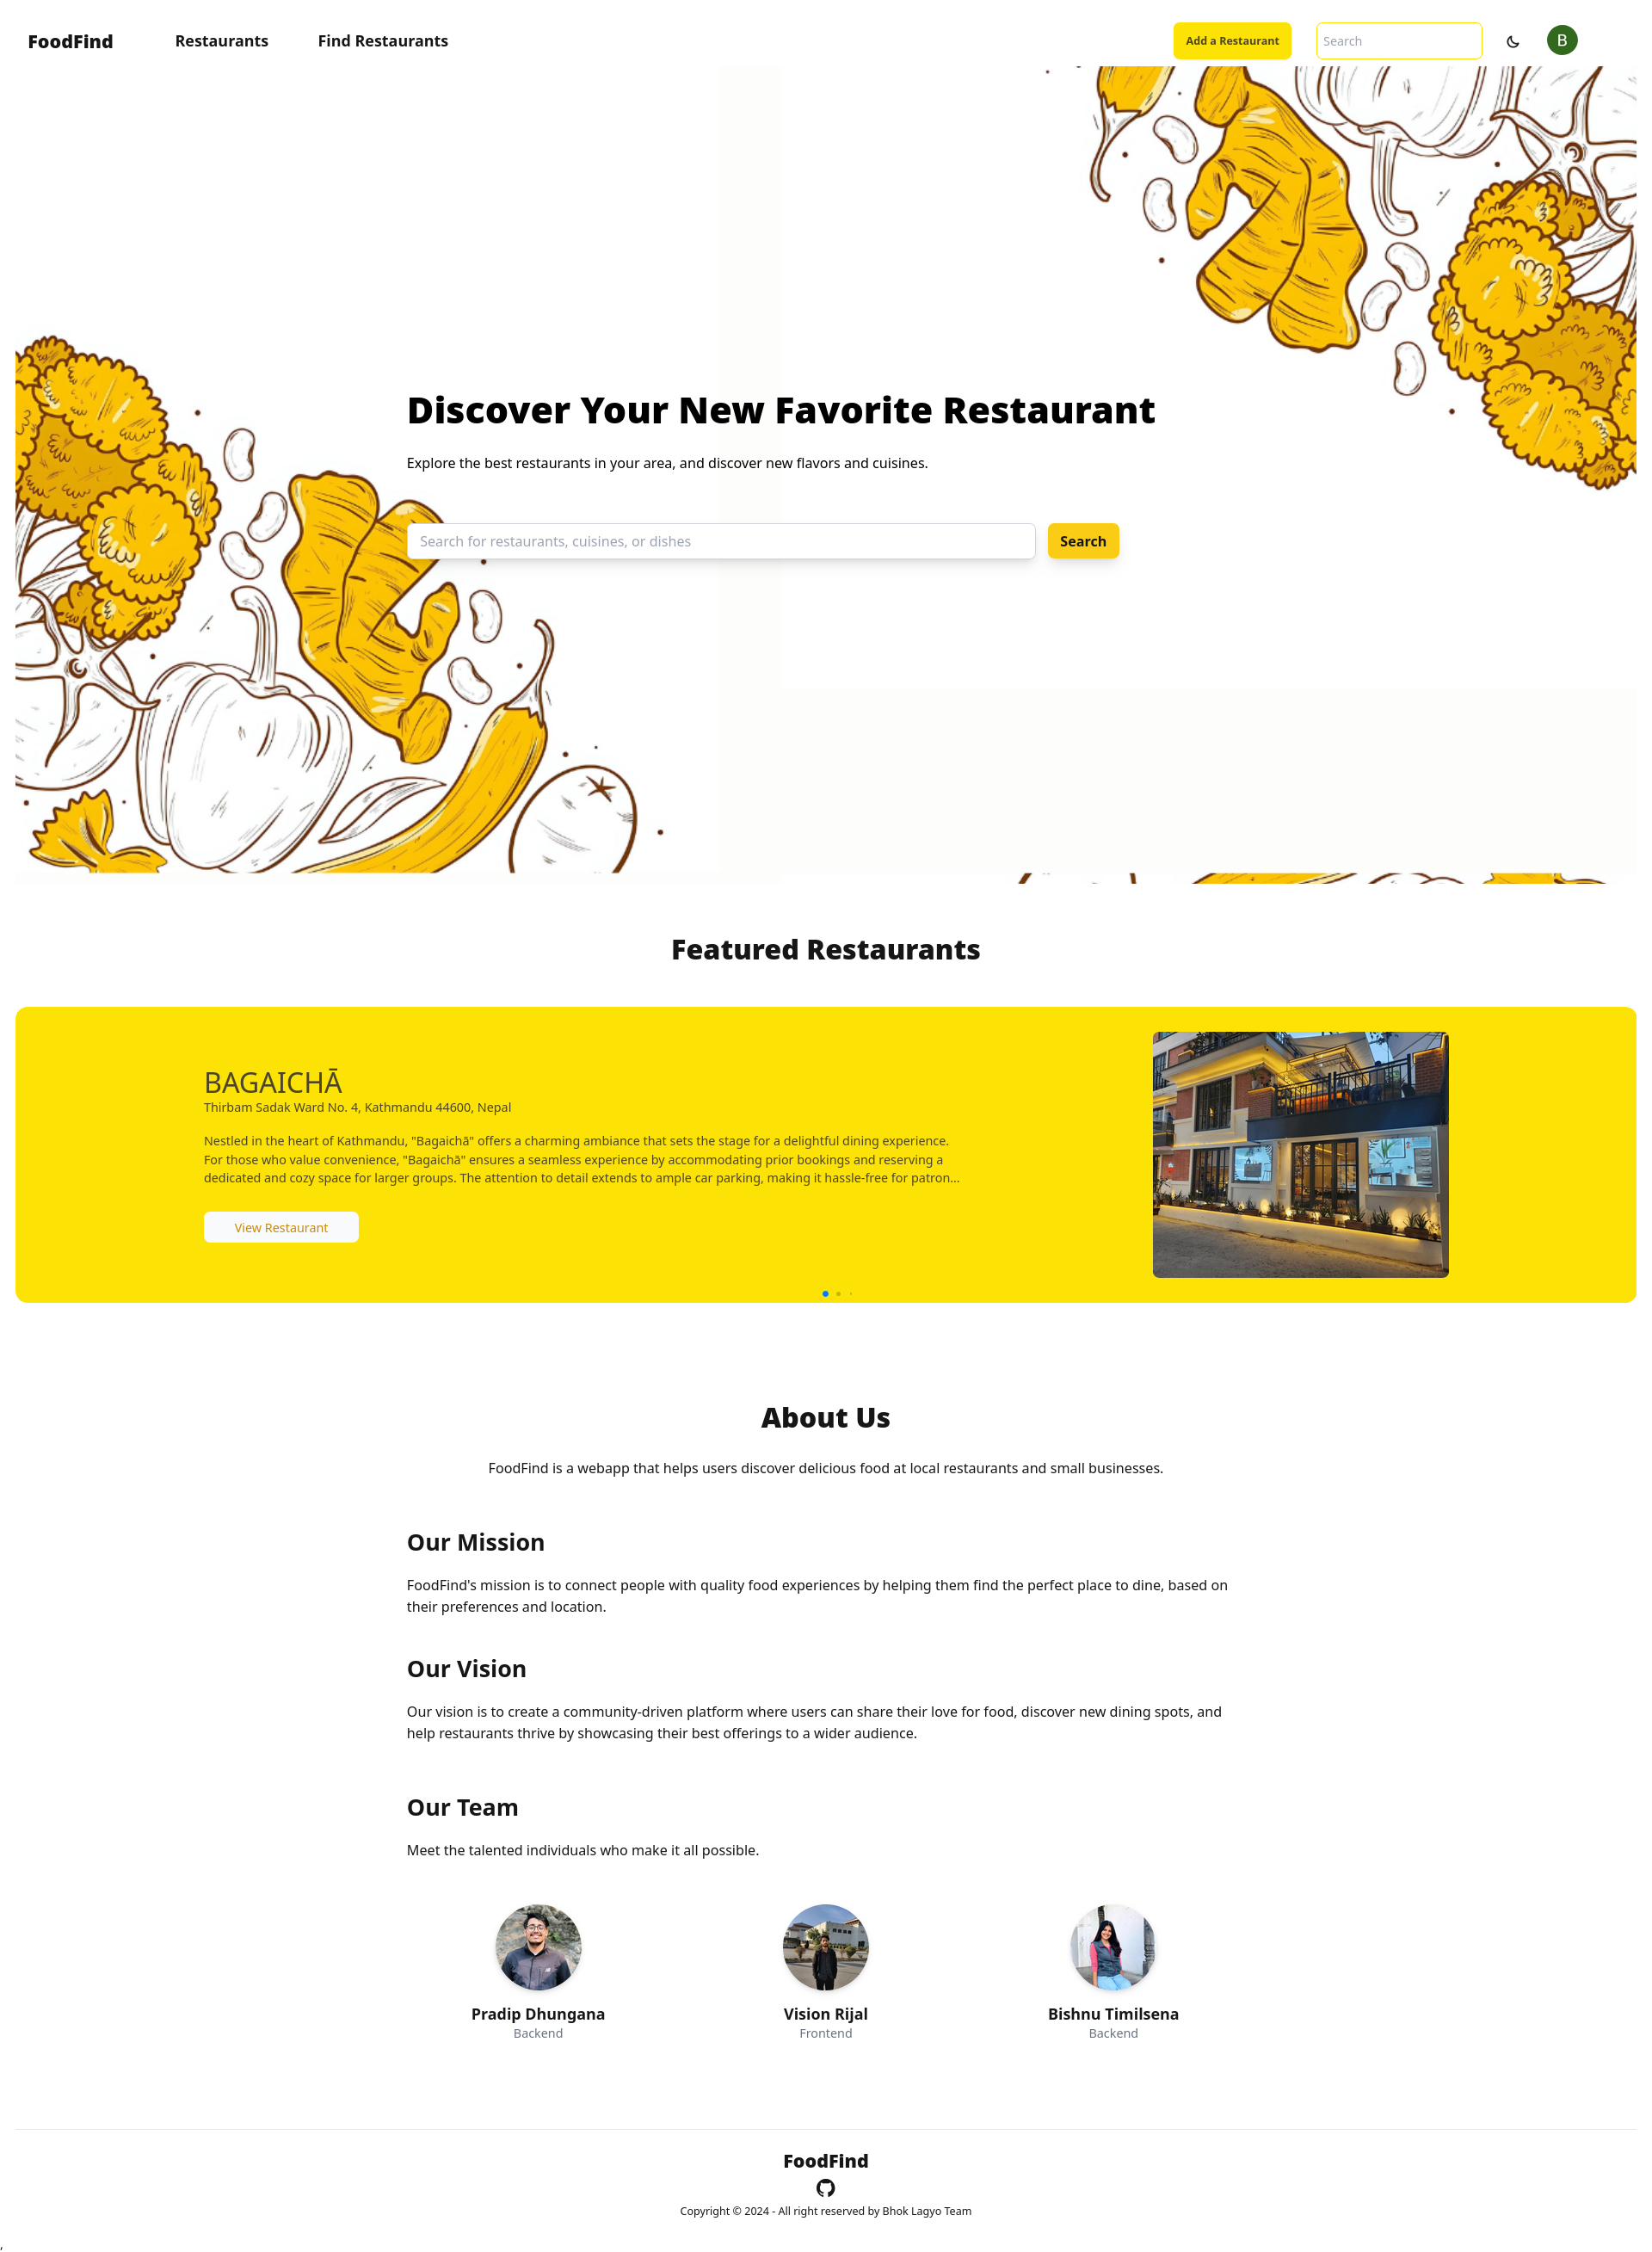
\includegraphics[width=0.8\textwidth]{home}
	\centering
	\caption{Home Page}
	\label{fig:Home Page}
\end{figure}

\begin{figure}[h]
	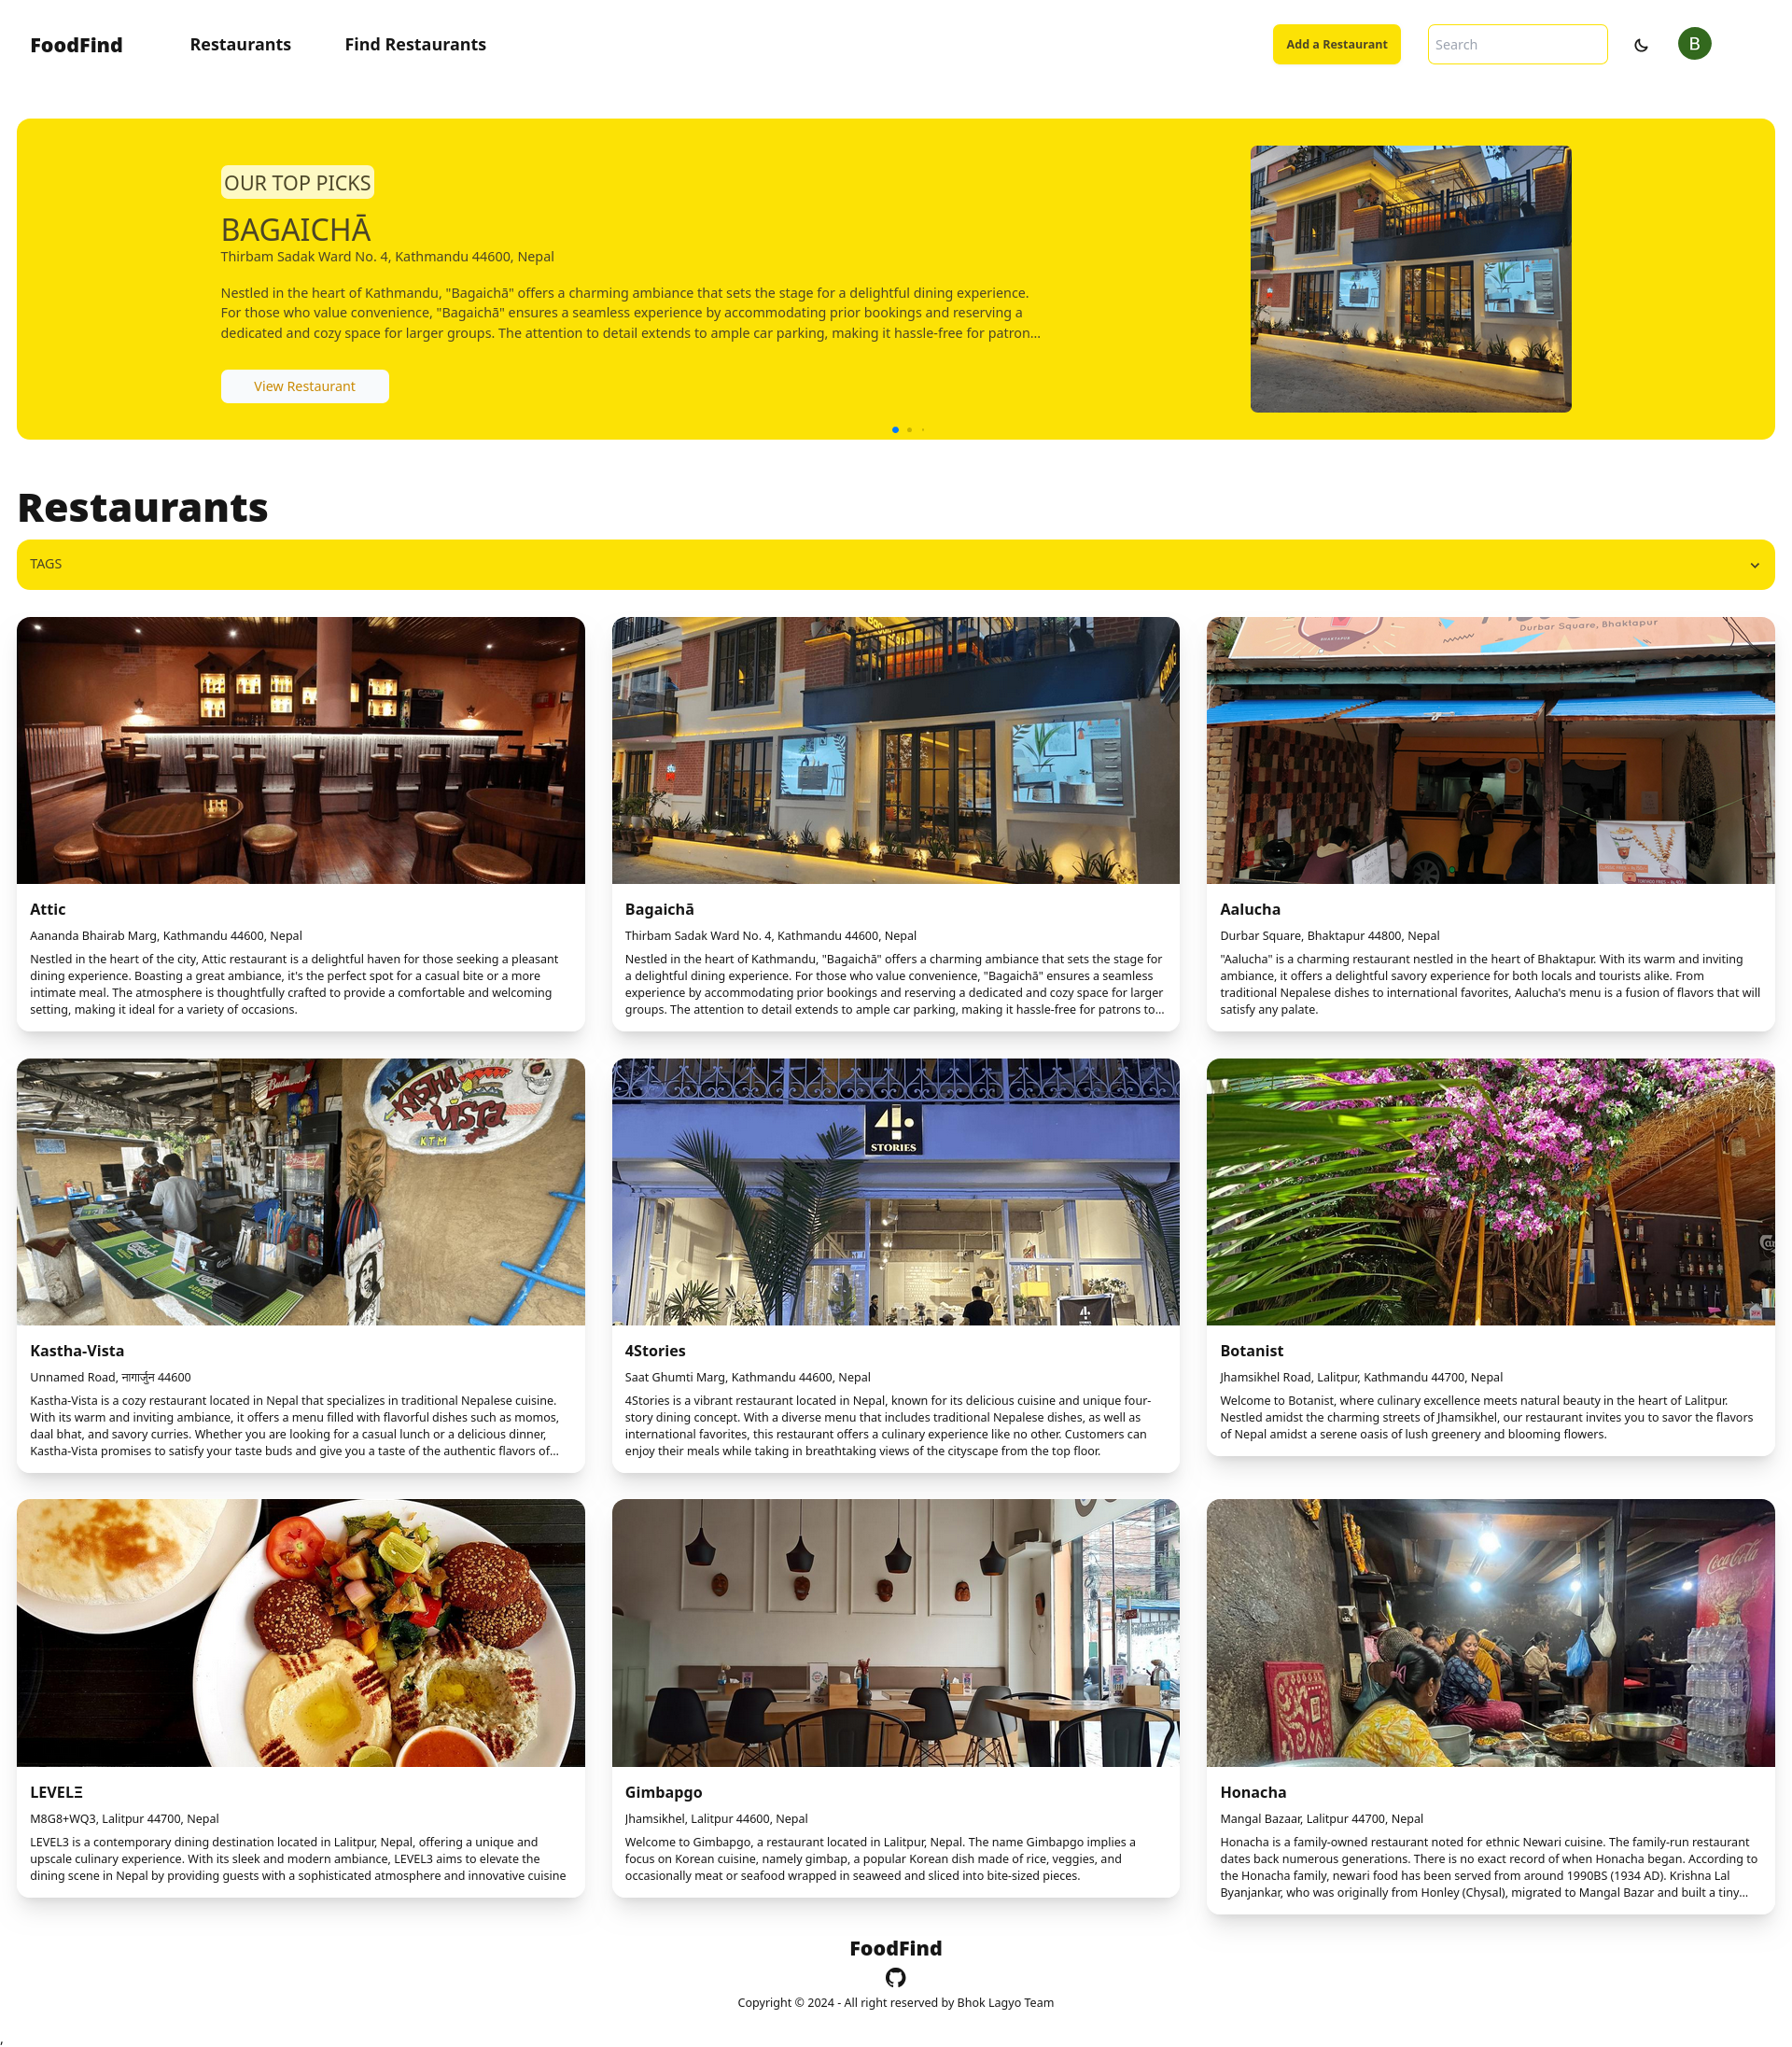
\includegraphics[width=0.9\textwidth]{restro}
	\centering
	\caption{Restaurants List}
	\label{fig:Restaurant}
\end{figure}

\vspace{7mm}
\begin{figure}[h]
	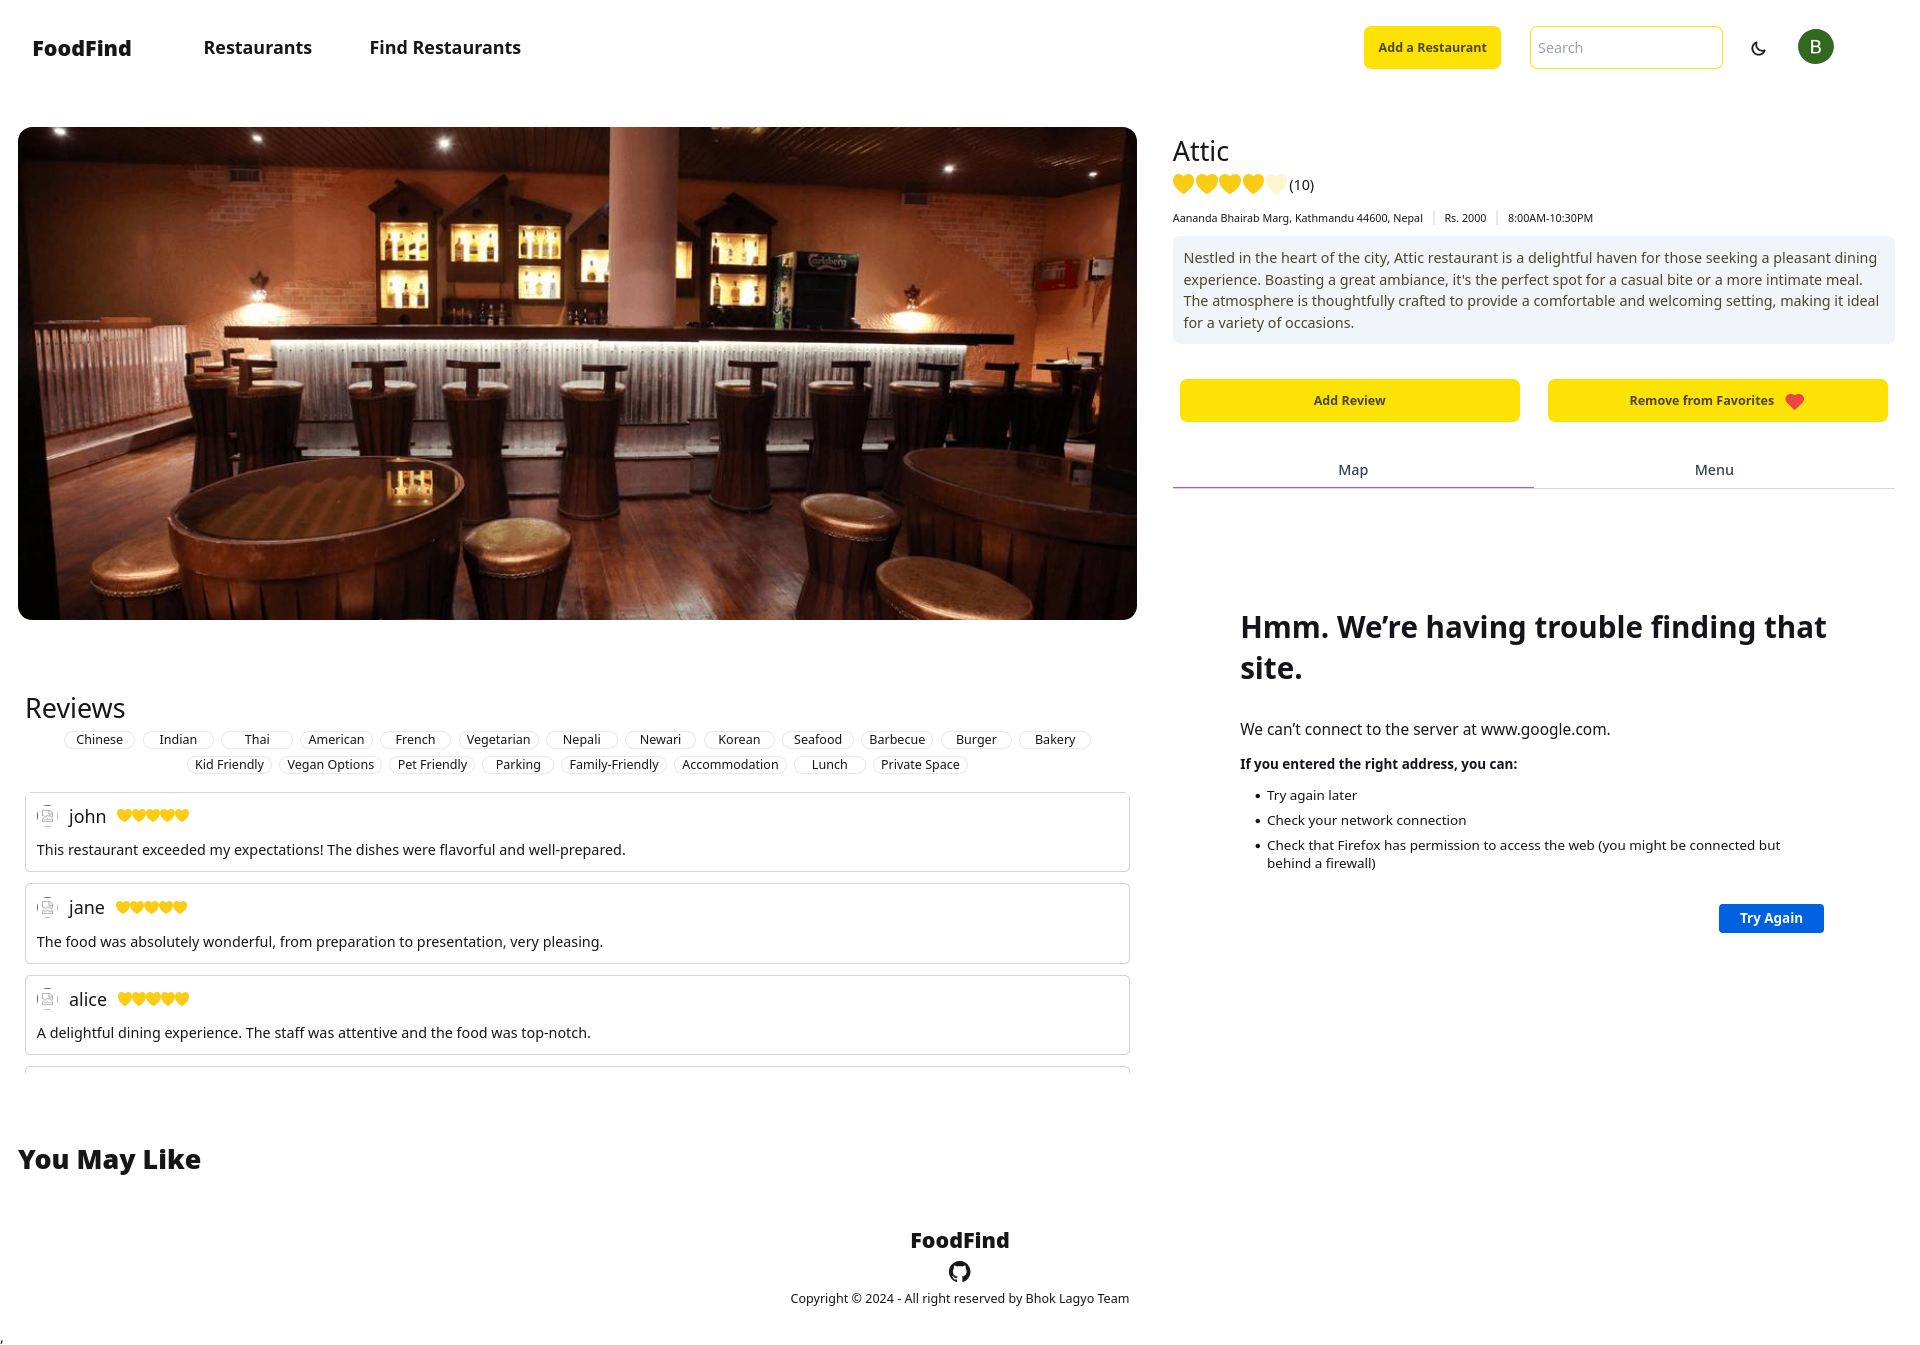
\includegraphics[width=0.8\textwidth]{profile}
	\centering
	\caption{Restaurant Profile}
	\label{fig:Profile}
\end{figure}

\vspace{7mm}
\begin{figure}[h]
	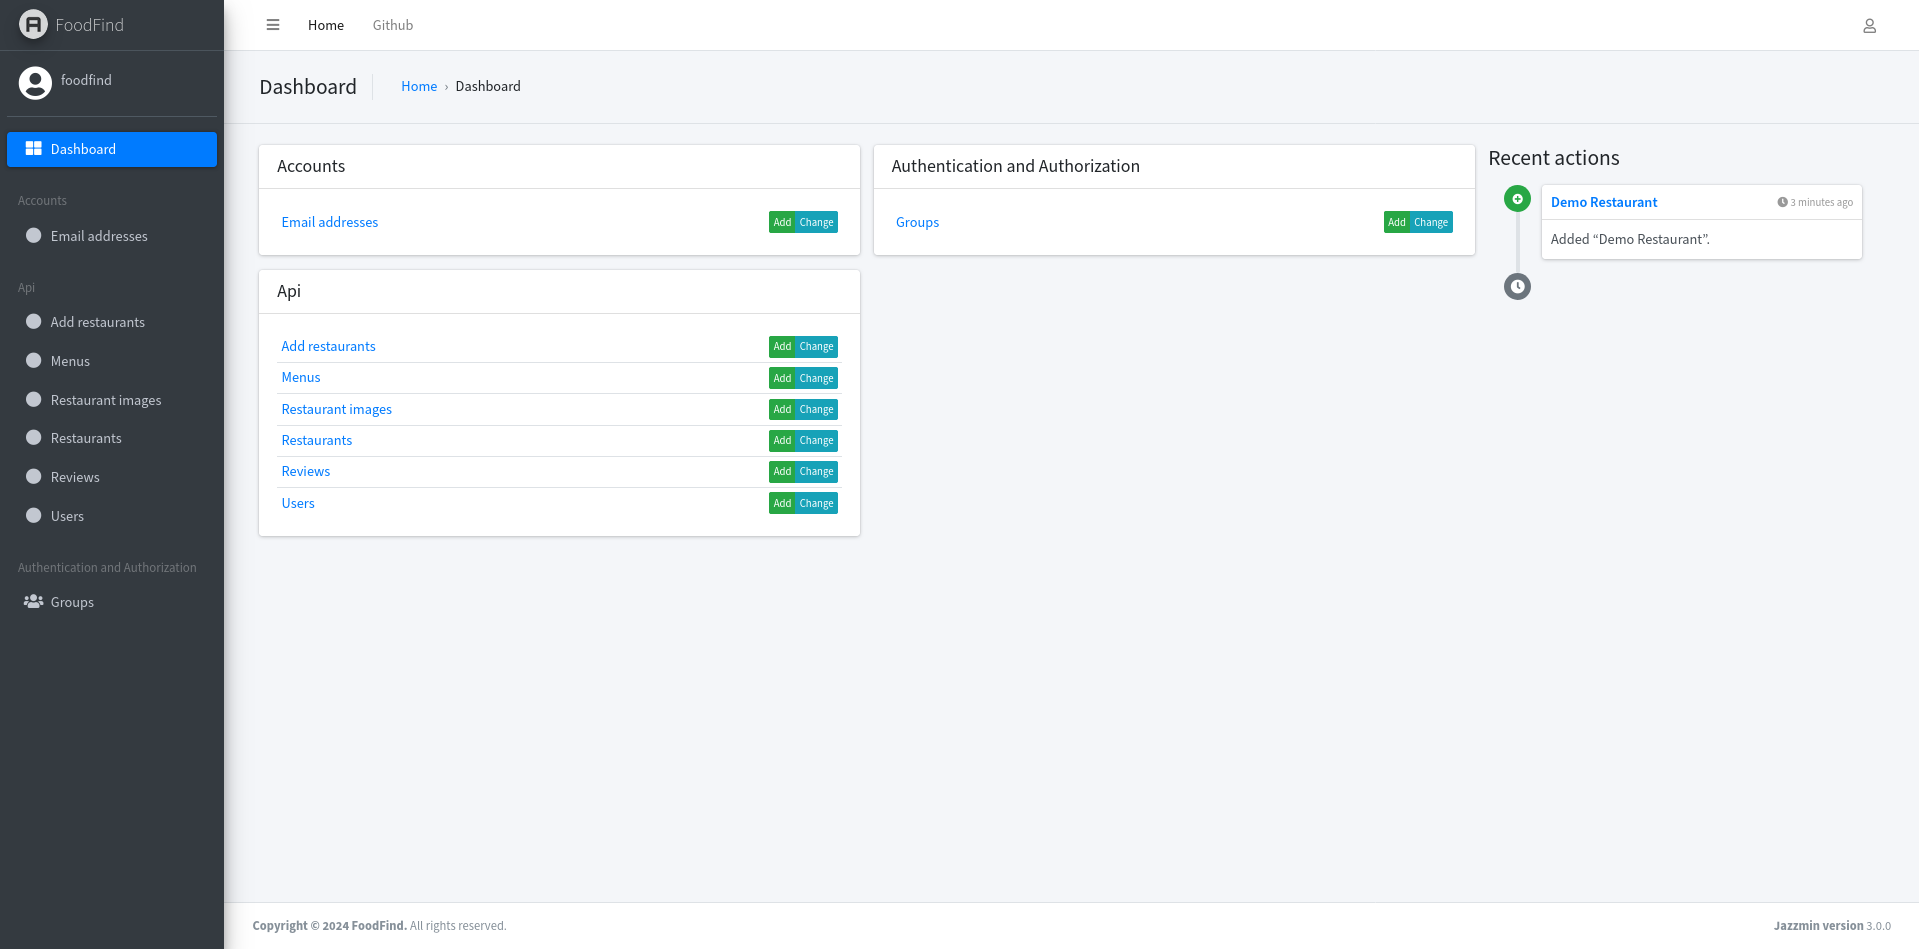
\includegraphics[width=0.8\textwidth]{admin}
	\centering
	\caption{Admin Section}
	\label{fig:Admin Section}
\end{figure}









\end{document}